%Version 3.1 December 2024
% See section 11 of the User Manual for version history
%
%%%%%%%%%%%%%%%%%%%%%%%%%%%%%%%%%%%%%%%%%%%%%%%%%%%%%%%%%%%%%%%%%%%%%%
%%                                                                 %%
%% Please do not use \input{...} to include other tex files.       %%
%% Submit your LaTeX manuscript as one .tex document.              %%
%%                                                                 %%
%% All additional figures and files should be attached             %%
%% separately and not embedded in the \TeX\ document itself.       %%
%%                                                                 %%
%%%%%%%%%%%%%%%%%%%%%%%%%%%%%%%%%%%%%%%%%%%%%%%%%%%%%%%%%%%%%%%%%%%%%

%%\documentclass[referee,sn-basic]{sn-jnl}% referee option is meant for double line spacing

%%=======================================================%%
%% to print line numbers in the margin use lineno option %%
%%=======================================================%%

%%\documentclass[lineno,pdflatex,sn-basic]{sn-jnl}% Basic Springer Nature Reference Style/Chemistry Reference Style

%%=========================================================================================%%
%% the documentclass is set to pdflatex as default. You can delete it if not appropriate.  %%
%%=========================================================================================%%

%%\documentclass[sn-basic]{sn-jnl}% Basic Springer Nature Reference Style/Chemistry Reference Style

%%Note: the following reference styles support Namedate and Numbered referencing. By default the style follows the most common style. To switch between the options you can add or remove “Numbered” in the optional parenthesis. 
%%The option is available for: sn-basic.bst, sn-chicago.bst%  
 
\documentclass[referee,lineno,pdflatex,sn-nature]{sn-jnl}% Style for submissions to Nature Portfolio journals
%%\documentclass[pdflatex,sn-basic]{sn-jnl}% Basic Springer Nature Reference Style/Chemistry Reference Style
%%\documentclass[pdflatex,sn-mathphys-num]{sn-jnl}% Math and Physical Sciences Numbered Reference Style
%%\documentclass[pdflatex,sn-mathphys-ay]{sn-jnl}% Math and Physical Sciences Author Year Reference Style
%%\documentclass[pdflatex,sn-aps]{sn-jnl}% American Physical Society (APS) Reference Style
%%\documentclass[pdflatex,sn-vancouver-num]{sn-jnl}% Vancouver Numbered Reference Style
%%\documentclass[pdflatex,sn-vancouver-ay]{sn-jnl}% Vancouver Author Year Reference Style
%%\documentclass[pdflatex,sn-apa]{sn-jnl}% APA Reference Style
%%\documentclass[pdflatex,sn-chicago]{sn-jnl}% Chicago-based Humanities Reference Style

%%%% Standard Packages
%%<additional latex packages if required can be included here>

\usepackage{graphicx}%
\usepackage{multirow}%
\usepackage{amsmath,amssymb,amsfonts}%
\usepackage{amsthm}%
\usepackage{mathrsfs}%
\usepackage[title]{appendix}%
\usepackage{xcolor}%
\usepackage{textcomp}%
\usepackage{manyfoot}%
\usepackage{booktabs}%
\usepackage{algorithm}%
\usepackage{algorithmicx}%
\usepackage{algpseudocode}%
\usepackage{listings}%
\usepackage{tabularx} %
\usepackage{longtable}
\usepackage{ragged2e}
\usepackage{xltabular}

\newcolumntype{L}{>{\RaggedRight\hspace{0pt}}X} %
%%%%

%%%%%=============================================================================%%%%
%%%%  Remarks: This template is provided to aid authors with the preparation
%%%%  of original research articles intended for submission to journals published 
%%%%  by Springer Nature. The guidance has been prepared in partnership with 
%%%%  production teams to conform to Springer Nature technical requirements. 
%%%%  Editorial and presentation requirements differ among journal portfolios and 
%%%%  research disciplines. You may find sections in this template are irrelevant 
%%%%  to your work and are empowered to omit any such section if allowed by the 
%%%%  journal you intend to submit to. The submission guidelines and policies 
%%%%  of the journal take precedence. A detailed User Manual is available in the 
%%%%  template package for technical guidance.
%%%%%=============================================================================%%%%

%% as per the requirement new theorem styles can be included as shown below
\theoremstyle{thmstyleone}%
\newtheorem{theorem}{Theorem}%  meant for continuous numbers
%%\newtheorem{theorem}{Theorem}[section]% meant for sectionwise numbers
%% optional argument [theorem] produces theorem numbering sequence instead of independent numbers for Proposition
\newtheorem{proposition}[theorem]{Proposition}% 
%%\newtheorem{proposition}{Proposition}% to get separate numbers for theorem and proposition etc.

\theoremstyle{thmstyletwo}%
\newtheorem{example}{Example}%
\newtheorem{remark}{Remark}%

\theoremstyle{thmstylethree}%
\newtheorem{definition}{Definition}%

\raggedbottom
%%\unnumbered% uncomment this for unnumbered level heads

\begin{document}

\title[Comparing supervised machine learning algorithms for the prediction of partial arterial pressure of oxygen during craniotomy]{Comparing supervised machine learning algorithms for the prediction of partial arterial pressure of oxygen during craniotomy}\label{title}

\author[1,2,3]{\fnm{Andrea S} \sur{Gutmann}}\email{andrea.gutmann@med.uni-muenchen.de}

\author[3,4]{\fnm{Maximilian M} \sur{Mandl}}\email{mmandl@ibe.med.uni-muenchen.de}

\author[1]{\fnm{Clemens} \sur{Rieder}}\email{clemens.rieder@hcma.at}

\author[1]{\fnm{Dominik J} \sur{Hoechter}}\email{dominik.hoechter@med.uni-muenchen.de}

\author[1]{\fnm{Konstantin} \sur{Dietz}}\email{konstantin.dietz@med.uni-muenchen.de}

\author[3,5]{\fnm{Benjamin P} \sur{Geisler}}\email{ben.geisler@gmail.com}

\author[3,4]{\fnm{Anne-Laure} \sur{Boulesteix}}\email{boulesteix@ibe.med.uni-muenchen.de}

\author[1]{\fnm{Roland} \sur{Tomasi}}\email{roland.tomasi@med.uni-muenchen.de}

\author*[1,6]{\fnm{Ludwig C} \sur{Hinske}}\email{chinske@alum.mit.edu}

\affil[1]{\orgdiv{Department of Anaesthesiology}, \orgname{LMU University Hospital, LMU Munich}, \orgaddress{\city{Munich}, \country{Germany}}}

\affil[2]{\orgdiv{Pettenkofer School of Public Health}, \orgaddress{\city{Munich},  \country{Germany}}}

\affil[3]{\orgdiv{Institute for Medical Information Processing, Biometry and Epidemiology (IBE)}, \orgname{Faculty of Medicine, LMU Munich,}, \orgaddress{\city{Munich}, \country{Germany}}}

\affil[4]{\orgdiv{Munich Center of Machine Learning}, \orgname{LMU Munich}, \orgaddress{\city{Munich}, \country{Germany}}}

\affil[5]{\orgdiv{Department of Health Management and Health Economics}, \orgname{University of Oslo}, \orgaddress{\city{Oslo}, \country{Norway}}}

\affil[6]{\orgdiv{Institute for Digital Medicine}, \orgname{University Hospital of Augsburg}, \orgaddress{\city{Augsburg},  \country{Germany}}}



\abstract{\textbf{Background and Objectives:} Brain tissue oxygenation is usually inferred from arterial partial pressure of oxygen ($paO_2$), which is in turn often inferred from pulse oximetry measurements or other non-invasive proxies. Our aim was to evaluate the feasibility of continuous $paO_2$ prediction in an intraoperative setting among neurosurgical patients undergoing craniotomies with modern machine learning methods.\label{abstract}

\textbf{Methods:} Data from routine clinical care of lung-healthy neurosurgical patients were extracted from databases of the respective clinical systems and normalized. We used recursive feature elimination to identify relevant features for the prediction of $paO_2$. Six machine learning regression algorithms (gradient boosting, k-nearest neighbors, random forest, support vector, neural network, linear model with stochastic gradient descent) and a multivariable linear regression were then tuned and fitted to the selected features. A performance matrix consisting of Spearman’s $\rho$, mean absolute percentage error (MAPE), adjusted $R^2$, mean absolute error (MAE) and root mean squared error (RMSE) was finally computed based on the test set and used to compare and rank each algorithm.

\textbf{Results:} We analyzed N=4,175 patients with n=14,495 observations. Between 5 and 23 features were selected from the analysis of the training dataset comprising 3,131 patients with 10,896 observations. The best algorithm, a regularized linear model with stochastic gradient descent, could predict $paO_2$ values with adjusted $R^2$=0.76, Spearman’s $\rho$=0.83, MAPE=15.2 \% and RMSE=41.7 mmHg. Further improvement was possible by calibrating the algorithm with the first measured $paO_2/FiO_2$ ratio during surgery.

\textbf{Conclusion:} $PaO_2$ can be predicted by perioperative routine data in neurosurgical patients even before blood gas analysis. The prediction improves further when including the first measured $paO_2/FiO_2$ ratio, realizing quasi-continuous $paO_2$ monitoring.
}

\keywords{machine learning; paO2; craniotomy; blood gas analysis; arterial partial pressure of oxygen}

%%\pacs[JEL Classification]{D8, H51}

%%\pacs[MSC Classification]{35A01, 65L10, 65L12, 65L20, 65L70}

\maketitle


\section*{Abbreviations}\label{abb}
\begin{table}[h]
\begin{tabular}{|l|l|}
    \hline
    ABG & Arterial Blood Gas \\
    BM & Base Model \\
    BMI & Body Mass Index \\
    CI & Confidence Interval \\
    CV & Cross-Validation \\
    $FiO_2$ & Fraction of Inspired Oxygen \\
    GBR & Gradient Boosting for Regression \\
    IQR & Interquartile Range \\
    KNN & Regression based on k-nearest neighbors \\
    MAE & Mean Absolute Error \\
    MAPE & Mean Absolute Percentage Error \\
    MLP & Multi-layer Perceptron Regressor \\
    MLR & Multivariable ordinary least squares Linear Regression \\
    n & Number of Observations (multiple per surgery) \\
    N & Number of Surgeries \\
    nMAE & Negative Mean Absolute Error \\
    nMAPE & Negative Mean Absolute Percentage Error \\
    nRMSE & Negative RMSE \\
    p/F & $paO_2/FiO_2$ \\
    $paO_2$ & Partial Arterial Pressure of Oxygen  \\
    $pAO_2$ & Alveolar Oxygen Partial Pressure  \\
    Q1 / Q3 & First / Third Quartile \\
    RFE & Recursive Feature Elimination \\
    RFR & Random Forest Regressor \\
    RMSE & Root Mean Squared Error \\
    SGD & Linear model fitted by minimizing a regularized empirical loss with stochastic gradient descent \\
    $SpO_2$ & Peripheral Oxygen Saturation \\
    SVR & Epsilon-Support Vector Regression \\
    TM & Tuned Model \\
    \hline
\end{tabular}
\end{table}

%\begin{linenumbers}
\section{Introduction}\label{sec1}

It has long been known that brain tissue is exquisitely sensitive to decreased levels of blood oxygen, leading to potentially irreversible damage, including brain death within minutes \cite{Busl2010}. Consequently, hypoxemia has been the subject of extensive research since the mid-19\textsuperscript{th} century, enabling a deeper understanding of its mechanisms and the development of life-saving interventions \cite{Mach2011}. Hyperoxemia, an elevated level of oxygen in the blood, has been less extensively studied, even though it might occur very frequently in clinical practice through supplemental oxygen. In the last few years, however, it has been claimed in the literature that oxygen’s inherently reactive nature may damage lipids, proteins, nucleic acids, and thus hyperoxemia may lead to acute lung, kidney, and myocardial injury, increased mortality, pulmonary complications, and cardio- and cerebrovascular complications \cite{Mach2011,McIlroy2022,Weenink2020}. Suzuki et al. estimate that more than 80 \% of patients undergoing general anesthesia are exposed to amounts of supplemental oxygen exceeding levels necessary to maintain a normal blood oxygen saturation \cite{McIlroy2022,Suzuki2018}. Diagnosing hyperoxemia is more difficult as its initial symptoms - if any - may be vague \cite{Mach2011,Hafner2015}, and also because confirmation requires an arterial blood draw. In contrast, hypoxemia can often be diagnosed with peripheral pulse oximetry, which is non-invasive. Consequently, hyperoxemia is the subject of less extensive research. The lack of consensus regarding potential oxygen over-supplementation highlights the need for further research and guidelines in clinical practice \cite{Hafner2015,Altemeier2007,Singer2005,Bitterman2009,Calzia2010}. 

Arterial blood gas analysis (ABG) is performed during surgeries and in the intensive care unit, allowing the indirect monitoring of gas exchange in the lungs, tissue oxygenation, and oxygen consumption. However, these measurements are only valid at the time of each arterial blood draw, which, due to their invasive nature, is infrequently performed. To overcome this limitation, several approaches have been developed to achieve a non-invasive and continuous estimation of the partial oxygen pressure ($paO_2$) as a proxy for blood oxygenation \cite{Brown2017,Bou-Khalil2017,Sanz2015,Fried1994,Sharma2019,BahmaniBohloli2018,Boulain2016}. These methods estimate blood oxygenation using factors such as the fraction of inspired oxygen ($FiO_2$) and oxygen saturation ($SpO_2$) \cite{Brown2017,Bou-Khalil2017,Sanz2015,Gross1981}, the oxygen transfer slope and estimated membrane oxygen transfer \cite{Fried1994}, the alveolar gas equation ($pAO_2$) \cite{Sharma2019} or venous blood gas samples \cite{BahmaniBohloli2018, Boulain2016, Tavakol2013, Raoufy2011}. However, it is important to note that our analysis reveals that none of these methods demonstrate a particularly high level of precision, and they also exhibit other limitations, such as constraints related to the formula they utilize.

Machine learning algorithms may be able to overcome these limitations and potentially perform better when predicting outcomes based on a higher number of features, non-linear effects, and complex association patterns \cite{Senders2018,Chae2020,Heo2019}. 

\label{objectives}Given the brain tissue's sensitivity to hypoxia, neurosurgical patients may be regularly administered excessive amounts of oxygen to increase the margin of safety in case of an emergency \cite{Weenink2020}. This cohort consists of lung-healthy patients who undergo frequent BGAs compared to other interventions, providing a larger data pool. Therefore, our study aimed to demonstrate that machine learning algorithms outperform surrogate parameters or existing equations in calculating $paO_2$ values for neurosurgical patients, achieving a satisfiable range of error and good performance parameters. Additionally, we aimed to identify the most accurate machine learning algorithm for near-continuous prediction of $paO_2$ values.

\section{Materials and Methods}\label{sec2}
\subsection{Data and Data Preparation}\label{sec2.1}
The study was conducted as a single-center retrospective cohort study.  Before accessing the data, our protocol (submission 19-539) received approval from the University of Munich’s institutional review board and consent was waived. 

We included all patients at the University Hospital of Munich between January 1\textsuperscript{st} 2008 and December 31\textsuperscript{st} 2019 undergoing craniotomy as identified by the German surgical procedure classification \cite{Stausberg1998} codes 5-01 or 5-02 being at least 18 years old. Further inclusion criteria were as follows: receiving general anesthesia with endotracheal intubation, with documented anesthesia induction, incision, closure, and termination of anesthesia times, and having at least two perioperatively $paO_2$ measurements. In cases where a patient had undergone multiple surgeries, the one with most $paO_2$ measurements was included for analysis. The minimum number of patients required for the study was calculated applying the formula $N=\frac{L}{f^2}+k+1$, with $k=23$ (number of available features), $f^2=0.02$ (small effect) and $L=27.94$ for $\alpha=0.05$ and $beta=0.9$ \cite{Cohen2013a, Cohen2013b}.

Data were extracted and integrated from the Anesthesia Information Management System (NarkoData\textregistered, IMESO IT GmbH, Giessen, Germany) and the Hospital Information System (SAP/Cerner i.s.h.med, Idstein, Germany) prior to data anonymization.

Hemoglobin and pH values were included regardless of their sampling site and without transformations \cite{AlEnezi2015,ref24}. Variables known to impact oxygenation were pre-selected. Additionally, we included the underlying physiologic model of the alveolar gas equation ($pAO_2$) \cite{Sharma2019} as well as the intraoperatively measured $paO_2/FiO_2$ (p/F) ratio as an indicator of pulmonary function. Ventilation compliance, represented by static compliance, was incorporated in our analysis as well \cite{Desai2019}. Finally, we calculated a $paO_2$ value based on Gadrey et al. \cite{Gadrey2019}. The formulas are stated in appendix \ref{secA1}. Each observation was defined as a set of multiple measurements at the same time, encompassing the aforementioned features, as well as one-time measures, such as socio-demographic information. The complete set of variables is provided in appendix \ref{secA2}. Of note, more than one observation was collected throughout each surgical procedure. Thus, multiple $paO_2$ values were predicted for each patient.

A detailed description of inclusion and exclusion criteria is provided in appendix \ref{secA3}.

After applying the exclusion criteria, no missing data were left.

All features (independent variables) and labels (dependent variable) were normalized before analysis by scaling them to a range between 0 and 1. The formula is stated in appendix \ref{secA1}. 

\subsection{Training and Test Datasets}\label{sec2.2}
The dataset was randomly divided by an 8:2 ratio into a training and test set, preventing an overoptimistic bias in performance evaluation. The feature selection process and hyperparameter tuning of all algorithms were conducted exclusively on the training set (Figure \ref{fig1}). The test set was reserved solely to calculate the performance metrics. The same set was used for evaluating feature importance, percentage errors and binning.

\begin{figure}[h]
\centering
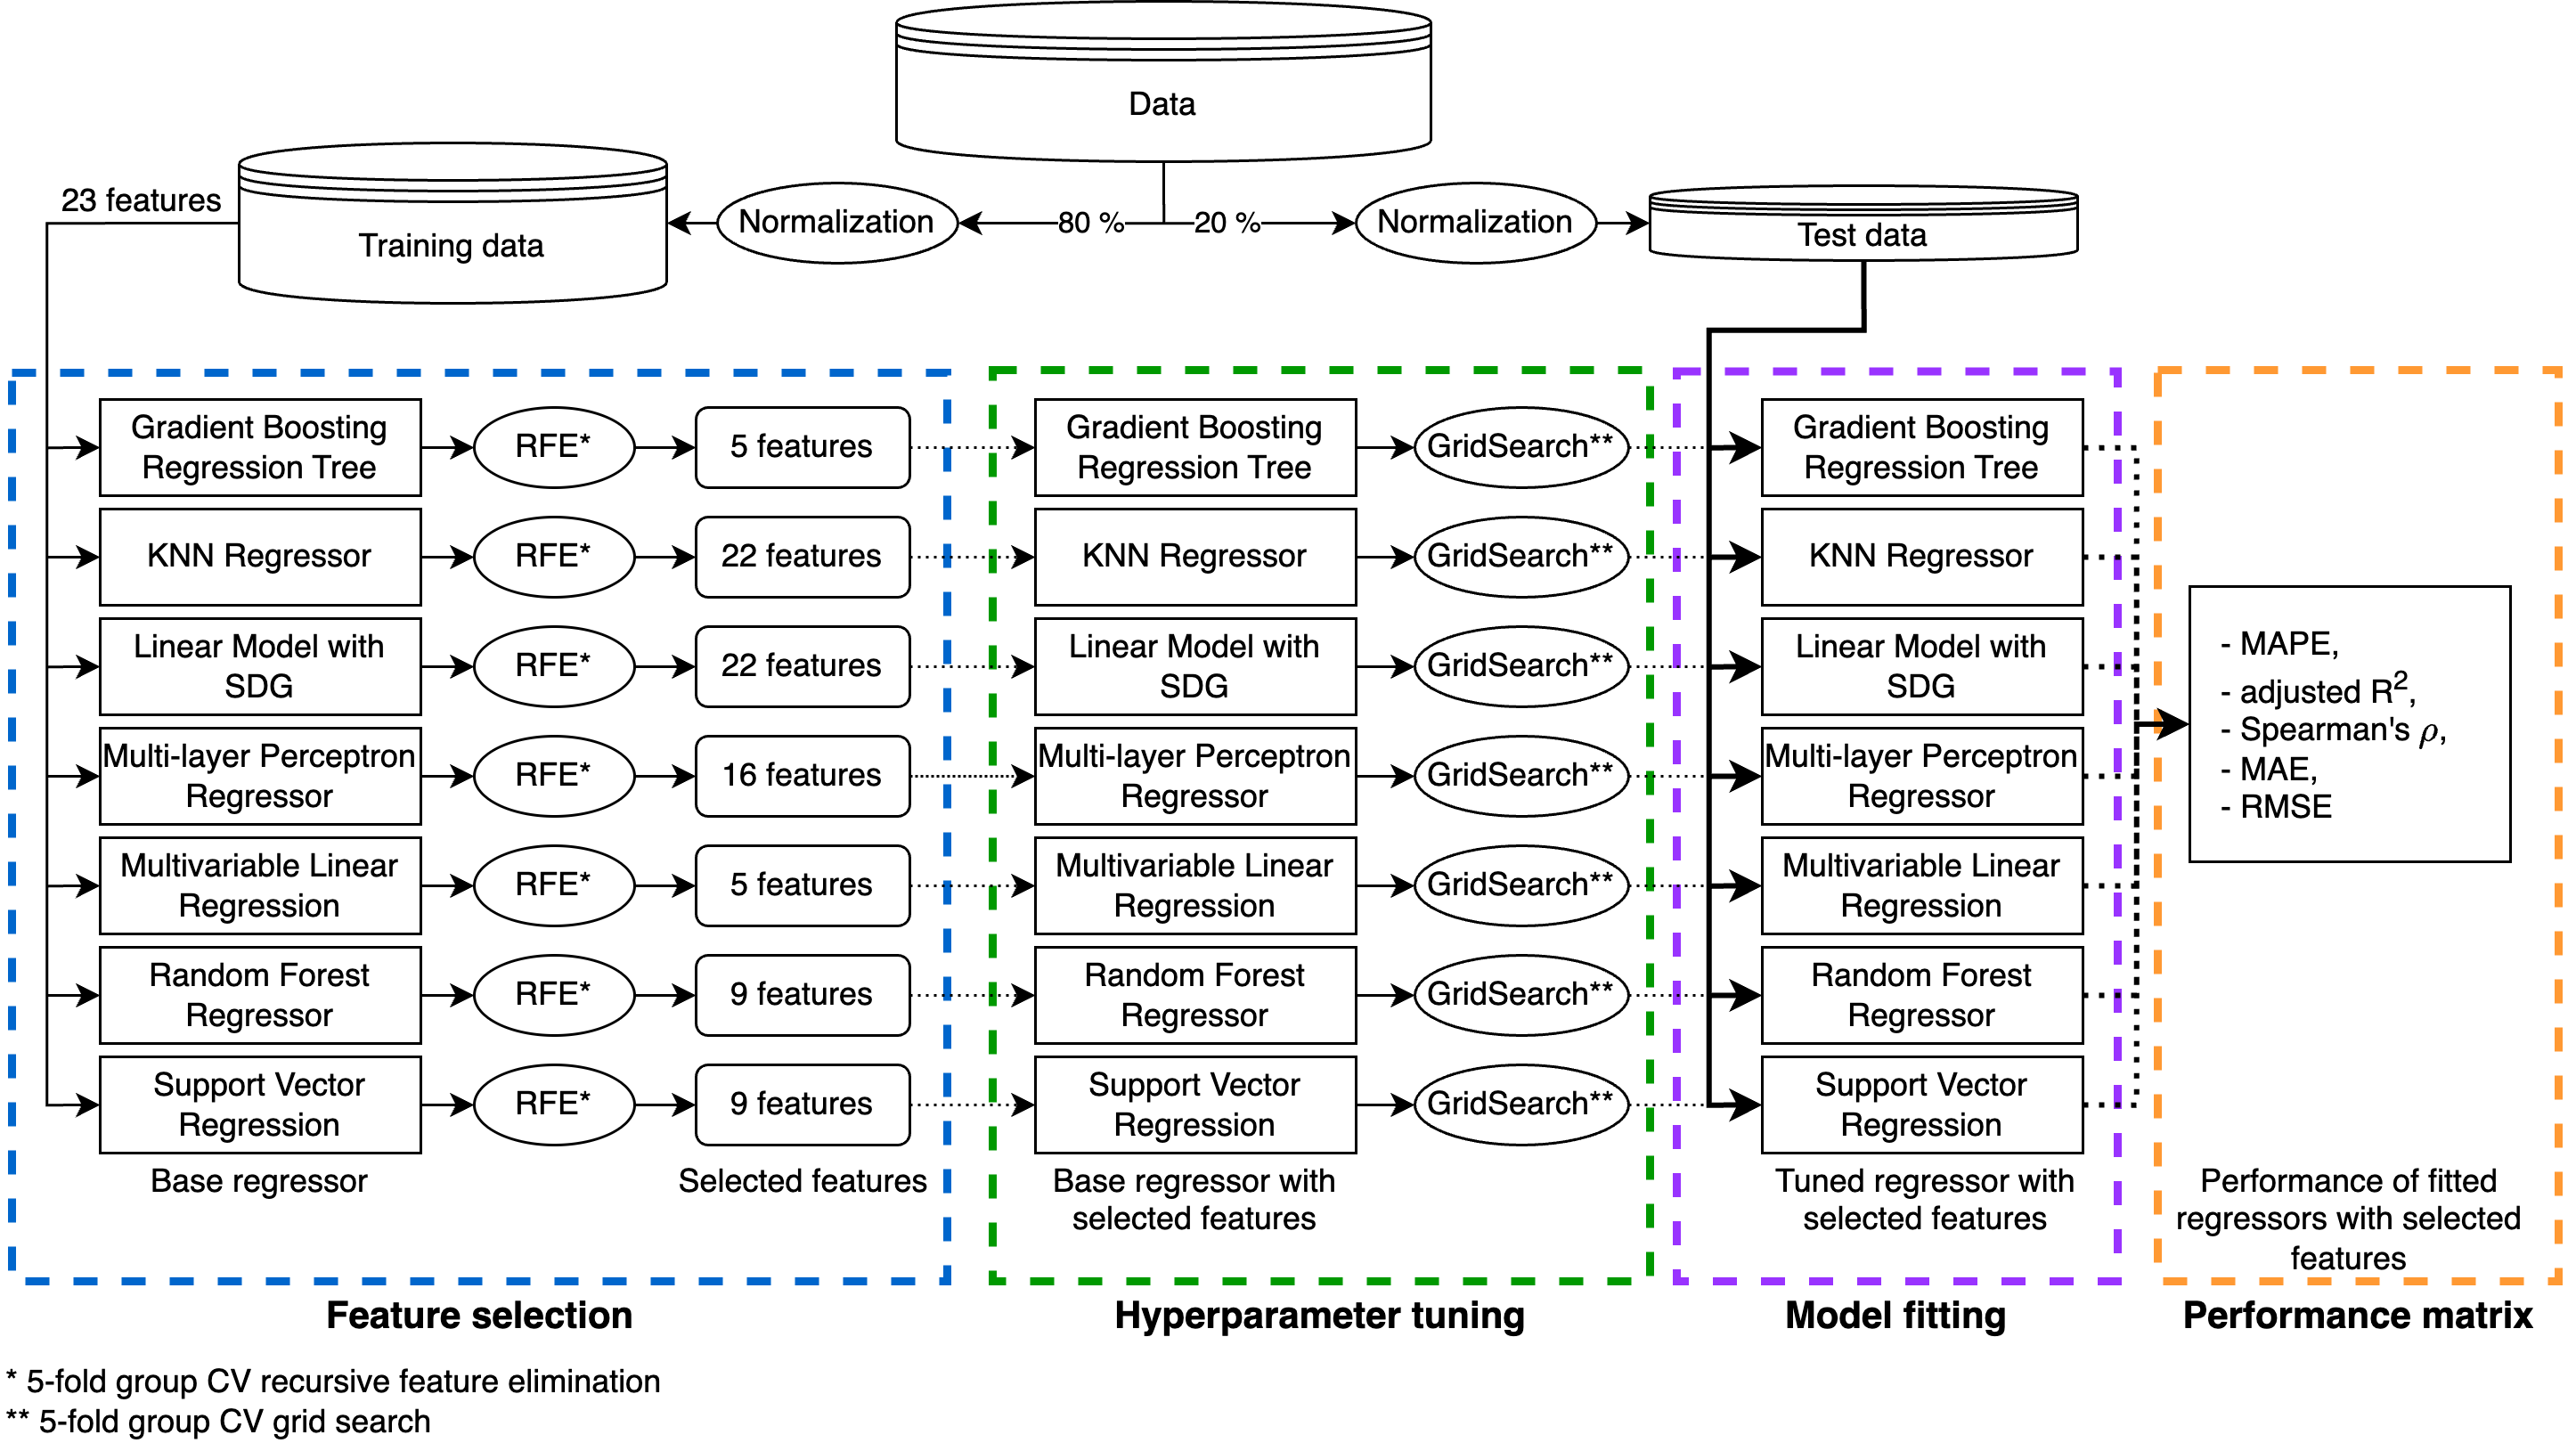
\includegraphics[width=0.9\textwidth]{images/Figure1.png}
\caption{\textbf{Methods Flowchart.} Use of data in training and testing during feature selection, hyperparameter tuning, model fitting and performance evaluation.}\label{fig1}
\end{figure}

\subsection{Feature Selection}\label{sec2.3}
To optimize each algorithm as effectively as possible, a separate feature selection was performed for each one separately. The optimal number of features was determined through a five-fold group cross-validation (CV) conducted on the training set, where each patient was randomly assigned to one of the five folds. The negative root mean squared error (nRMSE) was used as a performance metric. For the purpose of compatibility with the utilized package scikit-learn, performance metrics which should ideally be minimized (rather than maximized) were multiplied by -1. 

In addition to the employed machine learning algorithms (GBR, KNN, RFR, SVR, SGD, MLP), a multivariable linear regression (MLR) was used as a reference model. The optimal number of features for each regressor was selected by striking a balance between computational costs (number of features) and performance (cross-validated nRMSE scores), resulting in the requirement that all regressors achieve a nRMSE CV score of at least -0.081 mmHg. At this score, all algorithms demonstrated improvement, with four of them showing a substantial step increase. 

The feature selection was conducted using the recursive feature elimination (RFE), using each regressor as an estimator in turn. Feature ranking was calculated on the entire training set with the previously selected number of features to identify the most important ones. These features were subsequently used for hyperparameter tuning and fitting. 

\subsection{Tuning of Machine-Learning Algorithms and Model Fitting}\label{sec2.4}
Hyperparameter tuning was performed using a five-fold group cross-validation with a grid search approach, i.e., a search over all (combinations of) prespecified parameter values within the training set. For each algorithm, we performed a five-fold CV within each hyperparameter combination. For each fold, the nRMSE, the adjusted R2, the negative mean absolute percentage error (nMAPE), the negative mean absolute error (nMAE) and the times needed to fit and score each estimator were calculated. All these parameters were aggregated to their means and standard deviations per hyperparameter combination. The means of nRMSE, adjusted $R^2$, nMAPE, and nMAE were ranked among all hyperparameter combinations per algorithm.

The best model was selected as the one with the lowest sum of ranks for mean nRMSE, mean nMAPE, mean nMAE and mean adjusted $R^2$. If multiple models reached the same sum, the models were prioritized by the highest mean nRMSE, followed by the highest mean adjusted $R^2$ and the lowest mean scoring time. 

Details about the architectures of all algorithms are reported in appendix \ref{secA4}. 

\subsection{Performance Evaluation}\label{sec2.5}
For each base and tuned algorithm, a performance matrix consisting of five metrics was calculated on the whole test set. These metrics were (1) Spearman’s rank correlation coefficient $\rho$, (2) MAPE, (3) RMSE, (4) MAE, and (5) adjusted $R^2$ \cite{Sanz2015, Gadrey2019, Brown2016, Wu2020, Pedregosa2011}. 

For each algorithm, we ranked the quality measure of the tuned estimator from one for best to seven for worst based on the test set. These ranks were summed up as the overall rank for each algorithm, and the best one was determined by the lowest overall rank. 

\subsection{Further Evaluation}
Feature importance was evaluated using SHAP (SHapley Additive exPlanations) values \cite{Lundberg2017,Shapley1953}. 

We grouped all measured and predicted $paO_2$ values into bins spanning 50 mmHg based on the measured $paO_2$ value. Any values above 450 mmHg were grouped into a single bin, while all values below 100 mmHg were also grouped into a single bin. For each bin, the mean and standard deviation of the observed and the predicted $paO_2$ values was calculated. 

Outliers were defined based on a combination of the percentage errors ($PE=\frac{A_i-P_i*100}{A_i}$), the interquartile range (IQR), first quartile (Q1) and the third quartile (Q3): $outliers:=PE<[Q1-1.5*IQR; Q3+1.5*IQR]<PE$ \cite{Beniger1978}. We investigated all corresponding observations to detect differences between highly over- or underestimated $paO_2$ values. 

At last, the best algorithm was retrained with the first measured p/F ratio of each patient as an additional feature to assess whether the prediction of $paO_2$ values could be further improved. The same test set was used to calculate the performance measures.

\subsection{Implementation, Reproducibility, and Reporting}\label{sec2.6}
Data extraction, processing and analysis were done in Python on three different systems. Data were extracted on system 1, and statistical analyses were performed on system 2. All cross-validated recursive feature eliminations and grid searches were performed on system 3. Information about the systems and their operating systems as well as a complete list of each package version used in each system can be found in appendix \ref{secA5}. 

Extensive reporting for the prediction model development was done using the Transparent Reporting of a multivariable prediction model for Individual Prognosis Or Diagnosis checklist (appendix \ref{secA6}). The results of the study were reported following the guideline as provided by The Strengthening the Reporting of Observational Studies in Epidemiology in appendix \ref{secA7}.


\section{Results}\label{sec3}

\subsection{Patient Cohort}\label{sec3.1}
The calculated required sample size for the study was 1,421 patients. During the study period, 6,027 intracranial surgeries (number of surgeries, N) with 25,032 observations (number of perioperative value sets comprising two ABGs and all corresponding ventilation and surgical parameters as well as demographic data and vital signs, n) met the inclusion criteria. 10,537 observations and 1,852 surgeries were excluded based on our other criteria, resulting in a final data set of 4,175 surgeries with a total of 14,495 observations (appendix \ref{secA3}). The training set included 3,131 surgeries with 10,896 observations and the test set 1,044 surgeries with 3,599 observations.

The patients’ mean age was 54 years. Among the patients, 56 \% were female, and the mean body mass index (BMI) was 25.1 kg/m\textsuperscript{2}. The mean ventilation time was 357 min, the mean incision to closure time was 245 min. During ventilation time, every patient received on average 3.47 ABGs. The mean initial p/F ratio was 462.2. 156 patients had an American Society of Anesthesiologists (ASA) class of I, 1,643 had ASA class II, 1,941 had ASA class III, 400 had ASA class IV and 35 had ASA class V. The mean postoperative length-of-stay was 11.4 days. A detailed description as well as differences between the training and test set can be found in appendix \ref{secA8}.

\subsection{Feature Selection}\label{sec3.2}
The feature selection started with 23 variables (see appendix \ref{secA2}). The calculated nRMSE during cross-validated RFE for the scaled training set is shown in Figure \ref{fig2}. 

For every regressor, the highest nRMSE score was reached with 23 features. The appropriate number of features was selected at the first point at which the nRMSE exceeded -0.081 mmHg, which is indicated by the red vertical line on every plot in Figure \ref{fig2}.

\begin{figure}[h]
\centering
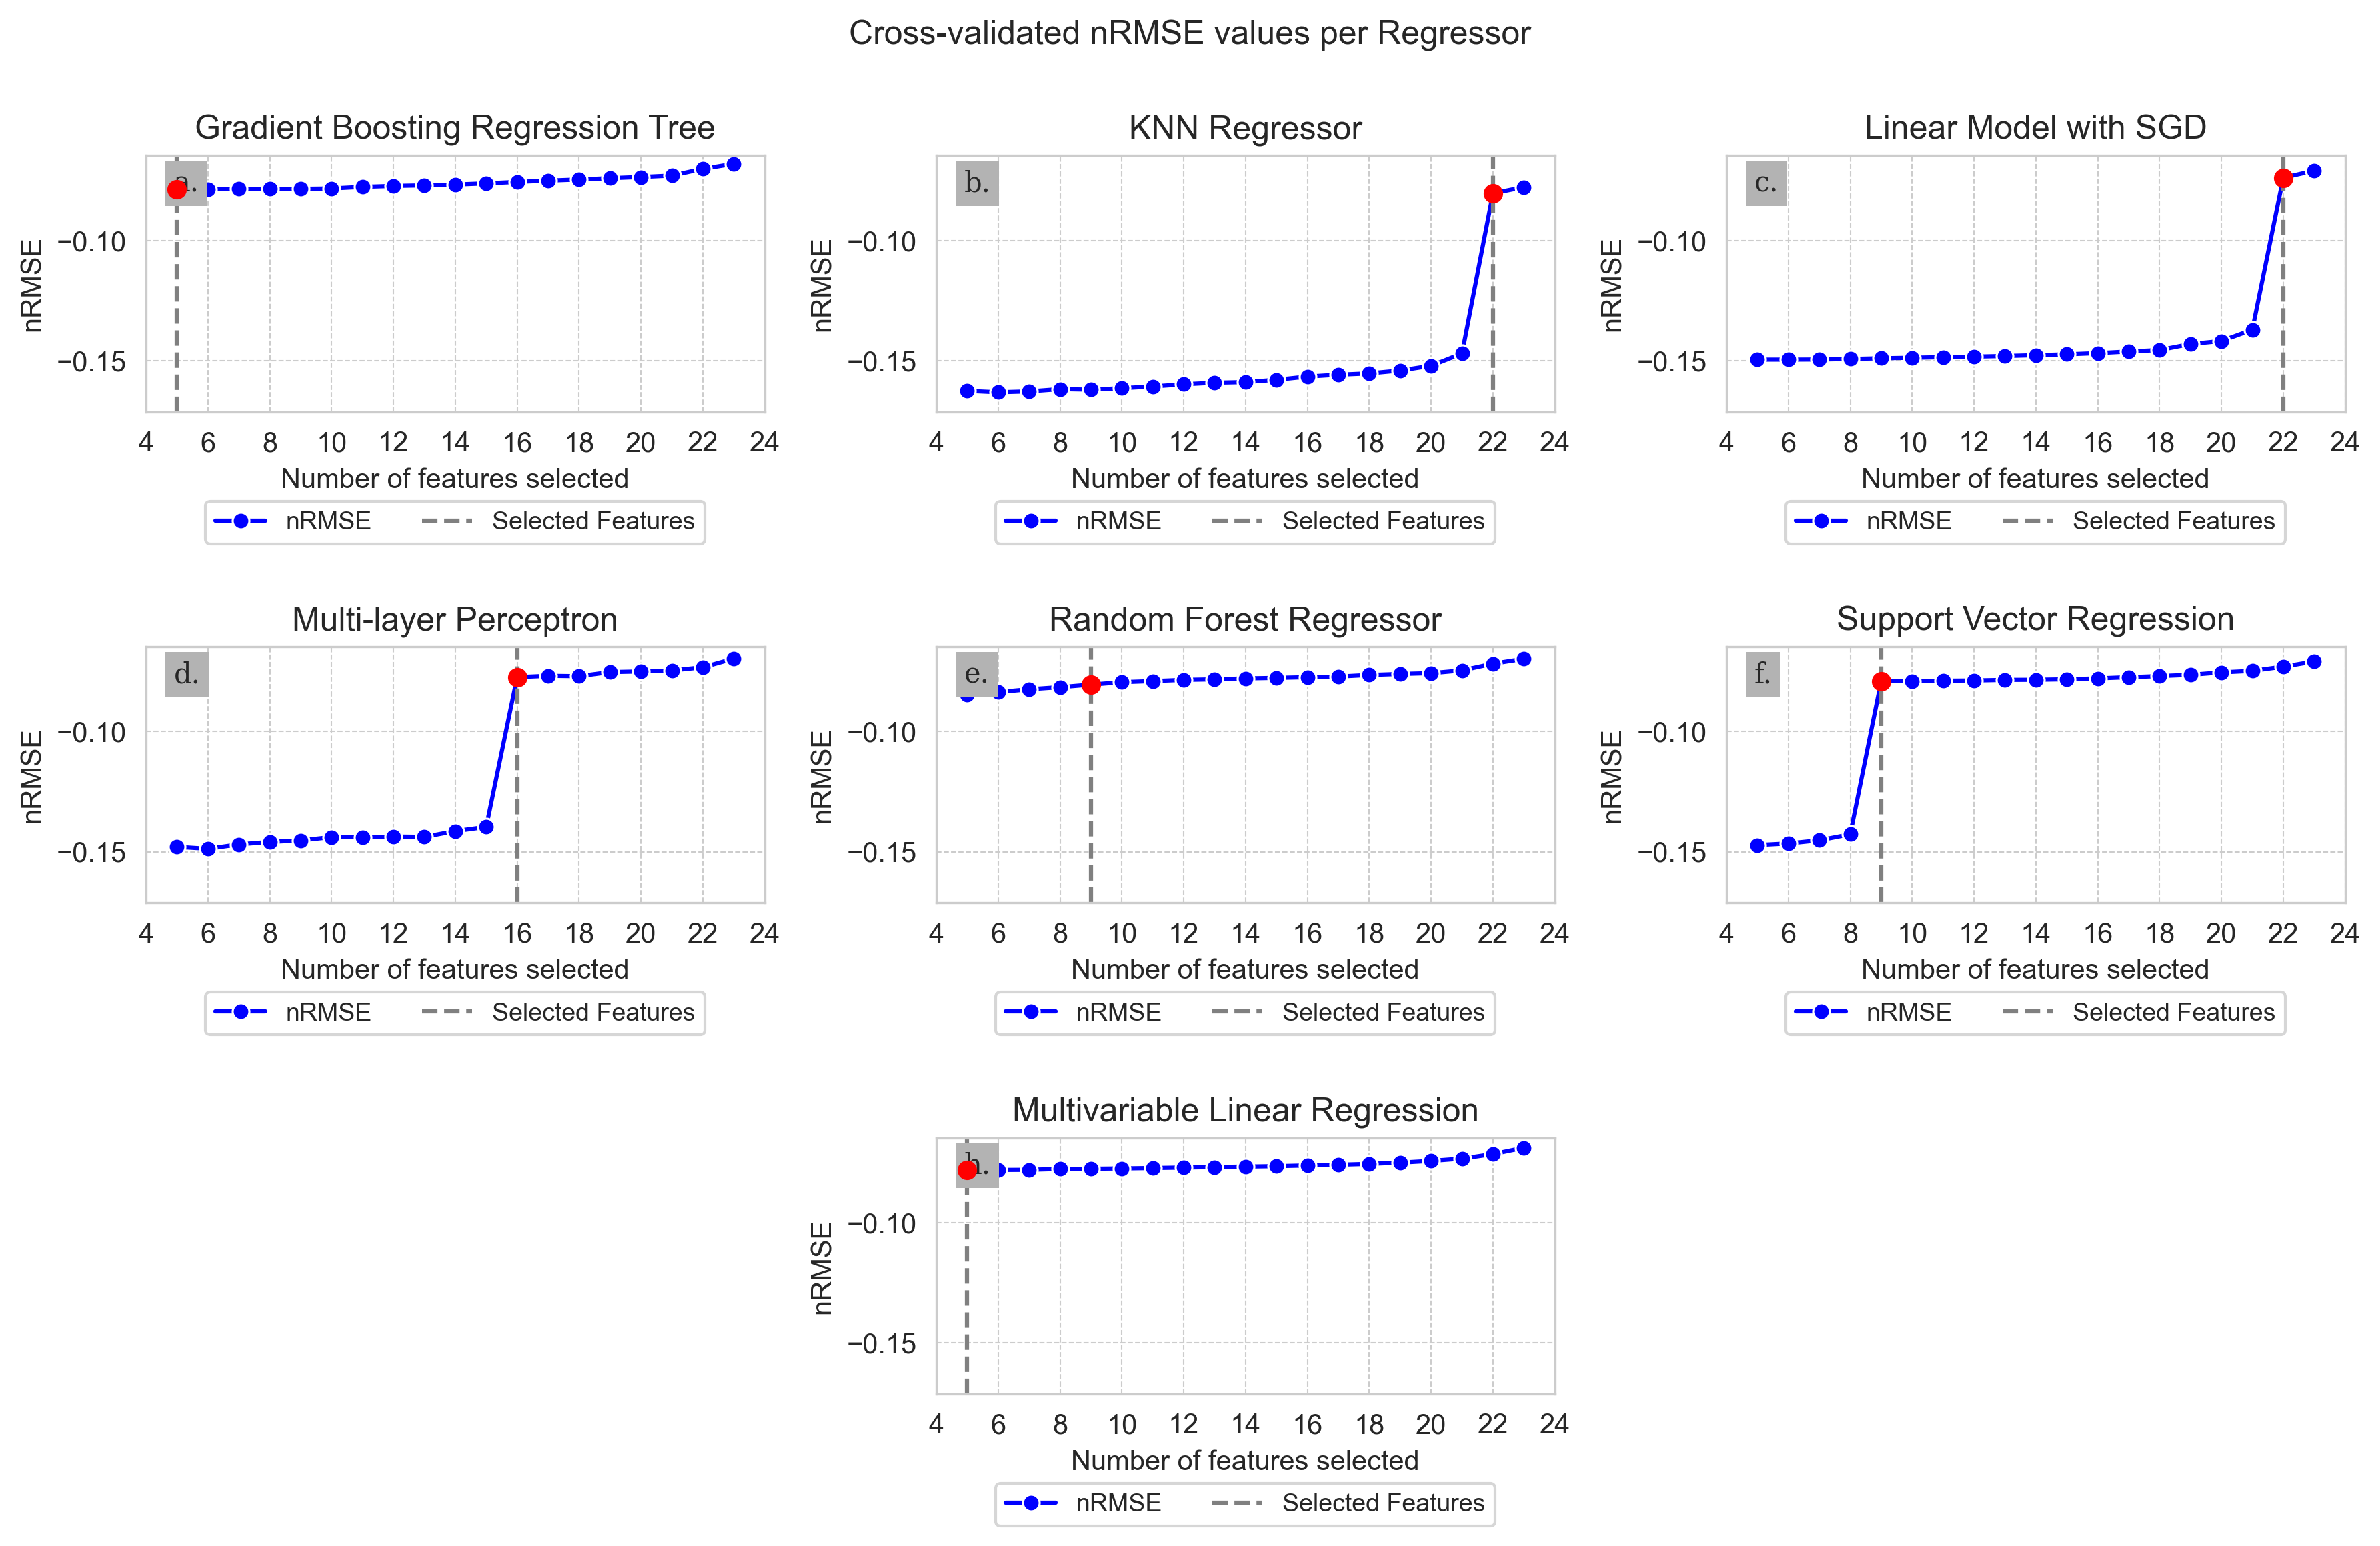
\includegraphics[width=0.9\textwidth]{images/Figure2.png}
\caption{\textbf{Cross-validation scores (nRMSE) for n number of features.} The red dot indicates the selected number of features.}\label{fig2}
\end{figure}


\subsection{Comparison to Popular Proxies and Base Regressors}\label{sec3.3}
The correlation coefficients of averaged $FiO_2$, $pAO_2$, and Gadrey's $paO_2$ to the averaged measured $paO_2$ were 0.73, 0.73 and 0.26 (Figure \ref{fig3}). 

\begin{figure}[h]
\centering
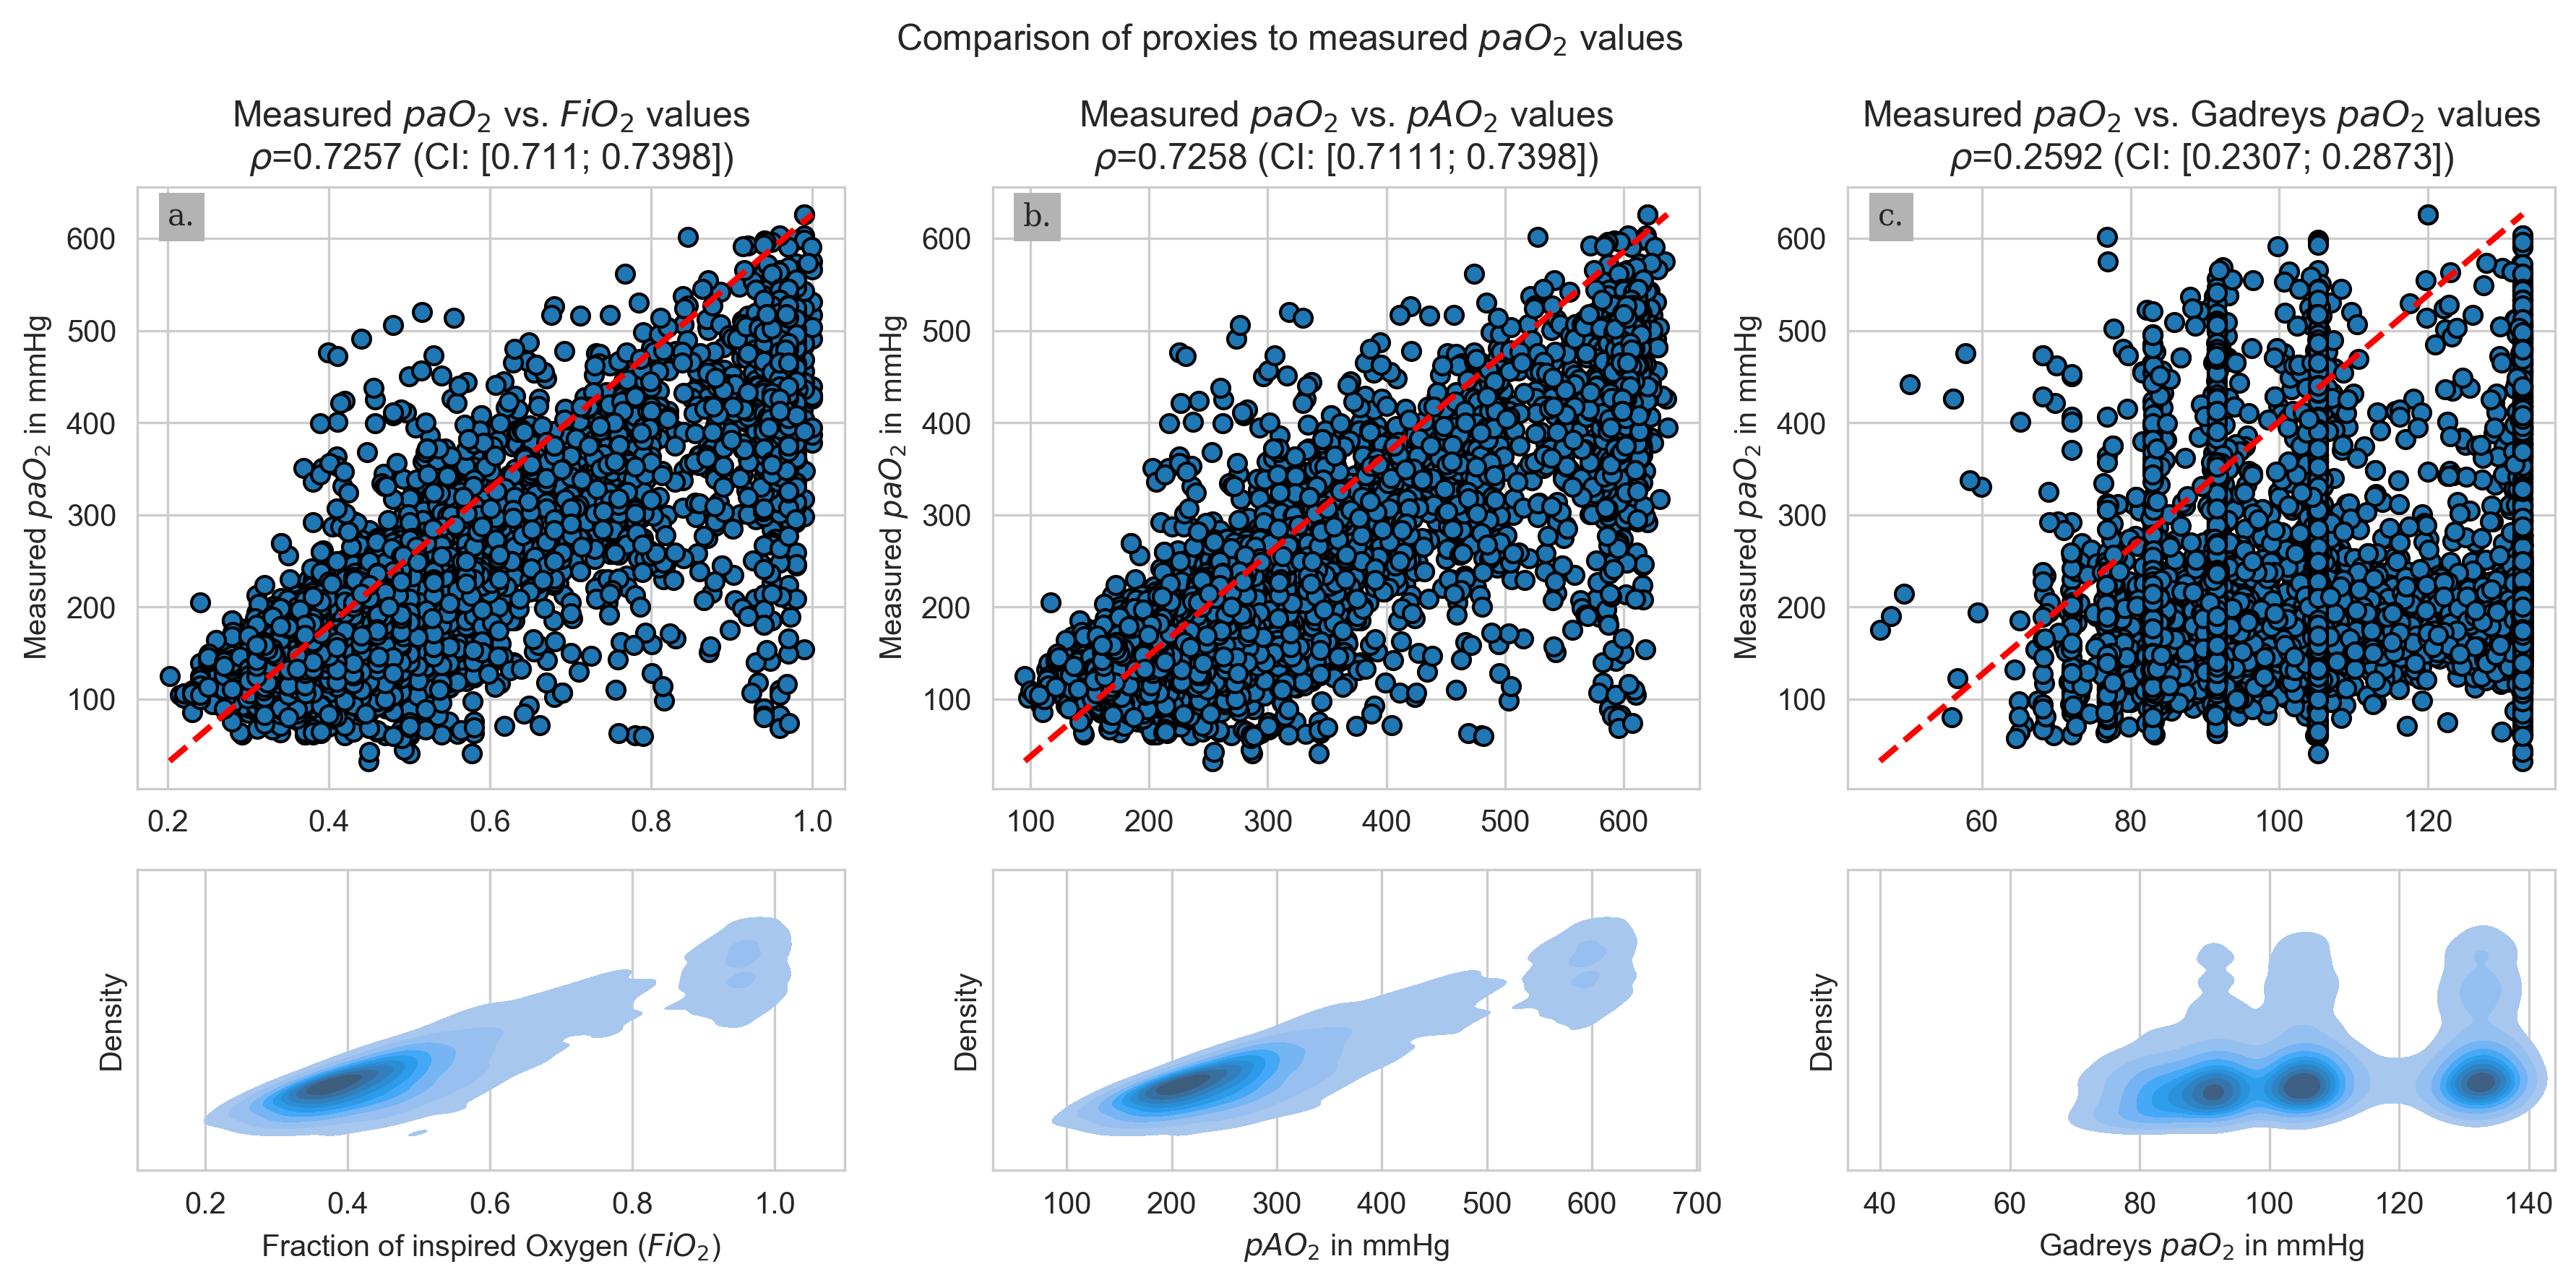
\includegraphics[width=0.9\textwidth]{images/Figure3.png}
\caption{\textbf{Comparison of $paO_2$ measurements to popular proxies.} The first row shows scatter plots of the parameter evaluated on the x-axis vs. the mean measured $pAO_2$ and the second row shows the density plots corresponding to the first row. First column: $FiO_2$; second column: $pAO_2$; third column: Gadrey’s $paO_2$.}\label{fig3}
\end{figure}

All base regressors for the $paO_2$ prediction (not-tuned regressors with default parameters) reached MAPEs between 16 and 20 \%, RMSEs of 50 mmHg and less (for rescaled data), MAEs of less than 79 mmHg (for rescaled data), adjusted $R^2$ between 0.66 and 0.74, correlation coefficients $\rho$ between 0.71 and 0.81 with confidence intervals ranging from 0.69 to 0.82. Therefore, all base regressors showed at least the same correlation coefficients between measured and predicted $paO_2$ values as the $FiO_2$ or $pAO_2$ values alone and a better correlation than Gadrey’s $paO_2$.

\subsection{Tuned Algorithms}\label{sec3.4}
After hyperparameter tuning, the GBR had an increased learning rate (0.2075) and decreased number of boosting stages (50). The minimum number of leaves for each tree was increased to three and the maximum depth decreased to two.

The tuned KNN used 21 neighbors and a BallTree algorithm to determine these neighbors. The used leaf size was decreased to 15. The Manhattan distance was used for the power parameter in the Minkowski metric.

The final RFR increased the number of trees to 200. The maximum tree depth was set to nine, and the maximum number of features considered for each tree decreased to four (log2). The minimum number of samples required for a split was increased to four and the function for quality measures of a split used the mean squared error with Friedman’s improvement score.

In the tuned SVR, the regularization parameter C decreased to 0.1. The tolerance for the stopping criterion increased to 0.01 and the cache size increased from 200 to 10,000. The shrinking heuristic was not used anymore. The kernel coefficient changed to 0.1.

The tuned SGD had a decreased constant for the multiplication of the regularization term of 0.00001. The squared error was used as a loss function with elasticnet as penalty. The Elastic Net Mixing parameter changed from 0.15 to 0.5. The learning rate changed to adaptive with an initial value of 0.1.

The tuned MLP had two hidden layers with 256 and 128 neurons. The activation function changed from a rectified linear unit function to a hyperbolic tan function. The size of the minibatch for stochastic optimizers was set to 128. The tolerance for optimization increased to 0.001, and early stopping was set to true. The maximum iteration increased from 200 to 350.

The MLR changed so that the coefficients were strictly positive and features may be overwritten during fitting.

All default and tuned parameters are listed in appendix \ref{secA4}.

\subsection{Performance Evaluation}\label{sec3.5}
The SGD reached the highest adjusted $R^2$ (0.76), the highest $\rho$ (0.83), the lowest MAPE (15.18 \%) and the lowest RMSE (41.69 mmHg), while it performed worse for the MAE (79.67 mmHg). Although most algorithms performed similarly, the SGD reached the lowest rank in four out of five parameters in our performance matrix from Table \ref{tab1}, and was hence selected as the best-performing algorithm for the given task.


\begin{sidewaystable}
\caption{Performance matrix of tuned algorithms.}\label{tab1}
\footnotesize{
\begin{tabular*}{\textheight}{@{\extracolsep\fill}llccccccc}
\toprule%
    & & GBR & KNN & MLP & MLR & RFR & SGD & SVR \\
\midrule
    \multirow{2}{*}{\textbf{Adjusted R$^2$}} 
    & BM & 0.6596 & 0.6892 & 0.7172 & 0.6580 & 0.6713 & 0.7375 & 0.6737 \\
    & TM & 0.6633 & 0.6977 & 0.7009 & 0.6589 & 0.6832 & \textbf{0.7566} & 0.6925 \\
    \# & & 6 & 3 & 2 & 7 & 5 & \textbf{1} & 4 \\
\midrule
    \multirow{2}{*}{\textbf{MAE in mmHg}} 
    & BM & 77.2 & 77.0 & 78.66 & 78.02 & 78.09 & 75.84 & 78.34 \\
    & TM & 77.18 & \textbf{72.51} & 78.19 & 77.83 & 77.01 & 79.67 & 77.88 \\
    \# & & 3 & \textbf{1} & 6 & 4 & 2 & 7 & 5 \\
\midrule
    \multirow{2}{*}{\textbf{MAPE in \%}} 
    & BM & 19.28 & 17.8 & 17.4 & 19.58 & 18.86 & 15.93 & 18.61 \\
    & TM & 19.28 & 17.23 & 18.02 & 19.55 & 18.45 & \textbf{15.18} & 18.21 \\
    \# & & 6 & 2 & 3 & 7 & 5 & \textbf{1} & 4 \\
\midrule
    \multirow{2}{*}{\textbf{RMSE in mmHg}} 
    & BM & 49.41 & 47.11 & 44.97 & 49.53 & 48.53 & 43.29 & 48.35 \\
    & TM & 49.14 & 46.45 & 46.25 & 49.47 & 47.64 & \textbf{41.69} & 46.94 \\
    \#  & & 6 & 3 & 2 & 7 & 5 & \textbf{1} & 4 \\
\midrule
    \multirow{4}{*}{\textbf{Spearman’s $\rho$}} 
    & \multirow{2}{*}{BM} & 0.7143  & 0.7752 & 0.7666 & 0.7101 & 0.7271 & 0.8282 & 0.7357 \\
    & & [0.698; 0.7300] & [0.7618; 0.7879] & [0.7528; 0.7798] & [0.6935; 0.7259] & [0.7113; 0.7421] & [0.8177; 0.8382] & [0.7203; 0.7503] \\
    & \multirow{2}{*}{TM} & 0.7138 & 0.782 & 0.7522 & 0.7100 & 0.7341 & \textbf{0.8282} & 0.7386  \\
    & & [0.6974; 0.7295] & [0.7689; 0.7943] & [0.7376; 0.7660] & [0.6934; 0.7258] & [0.7187; 0.7488] & \textbf{[0.8177; 0.8382]} & [0.7234; 0.7531] \\
    \#  & & 6 & 2 & 3 & 7 & 5 & \textbf{1} & 4 \\
\botrule
\end{tabular*}
}
\footnotetext{Adjusted $R^2$, MAE, MAPE, RMSE, and Spearman’s $\rho$ [95 \% CI] for each algorithm with default parameter values (Base Model (BM)) and tuned parameter values (Tuned Model (TM)) based on the test data set. The rank of the regressor for the considered performance metric is indicated in the column.}
\end{sidewaystable}

To visualize the correlation for each algorithm, the predicted and measured $paO_2$ values of the test set were plotted against each other (Figure \ref{fig4}). 

\begin{figure}[h]
\centering
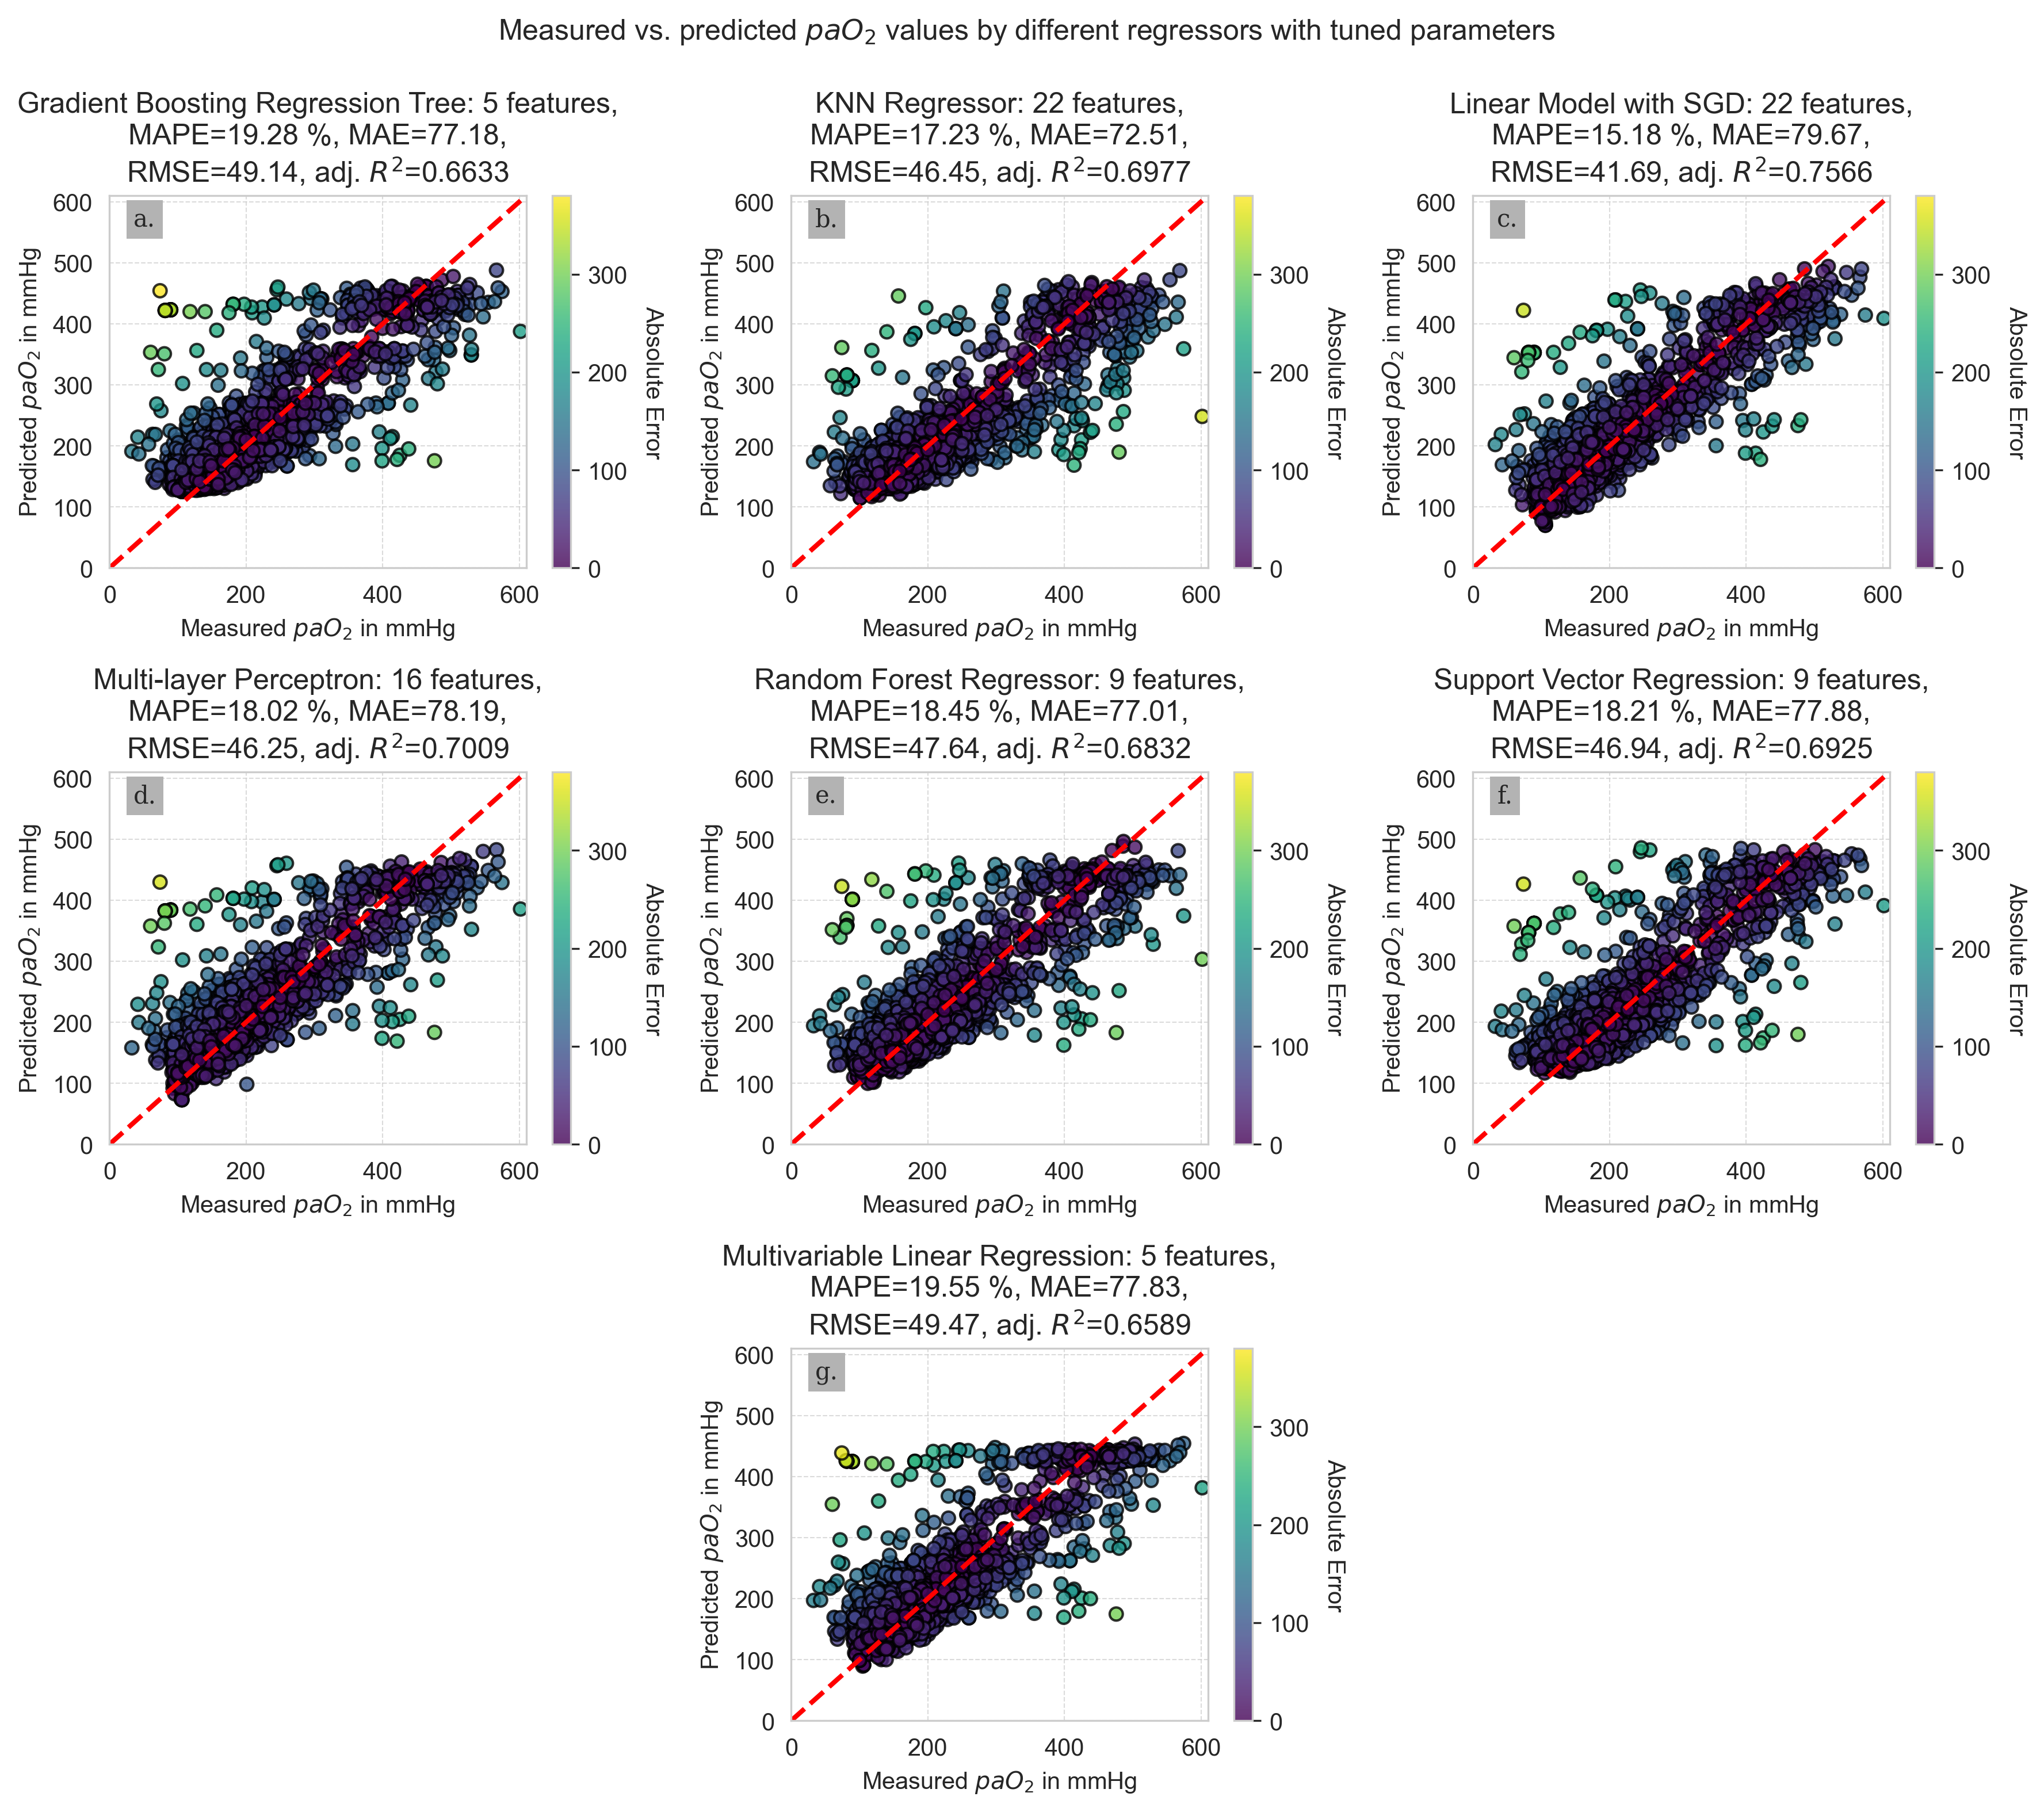
\includegraphics[width=0.9\textwidth]{images/Figure4.png}
\caption{\textbf{Scatterplots of measured vs. predicted paO2 values for different estimators.} a. Gradient Boosting for Regression, b. Regression based on k-nearest neighbors, c. Linear model fitted by minimizing a regularized empirical loss with stochastic gradient descent, d. Multi-layer Perceptron Regressor, e. Random Forest Regressor, f. Epsilon-Support Vector Regression, g. Multivariable ordinary least squares Linear Regression.}\label{fig4}
\end{figure}

\subsection{Further Evaluation}\label{sec3.6}
In the next step, we constructed a confusion matrix using the test set, with bins defined in 50 mmHg intervals. Values below 100 mmHg and above 450 mmHg were grouped into single bins at each extreme (Figure \ref{fig5}). Information about means and standard deviations for each bin is provided in table 2 (appendix \ref{secA9}).

\begin{figure}[h]
    \centering
    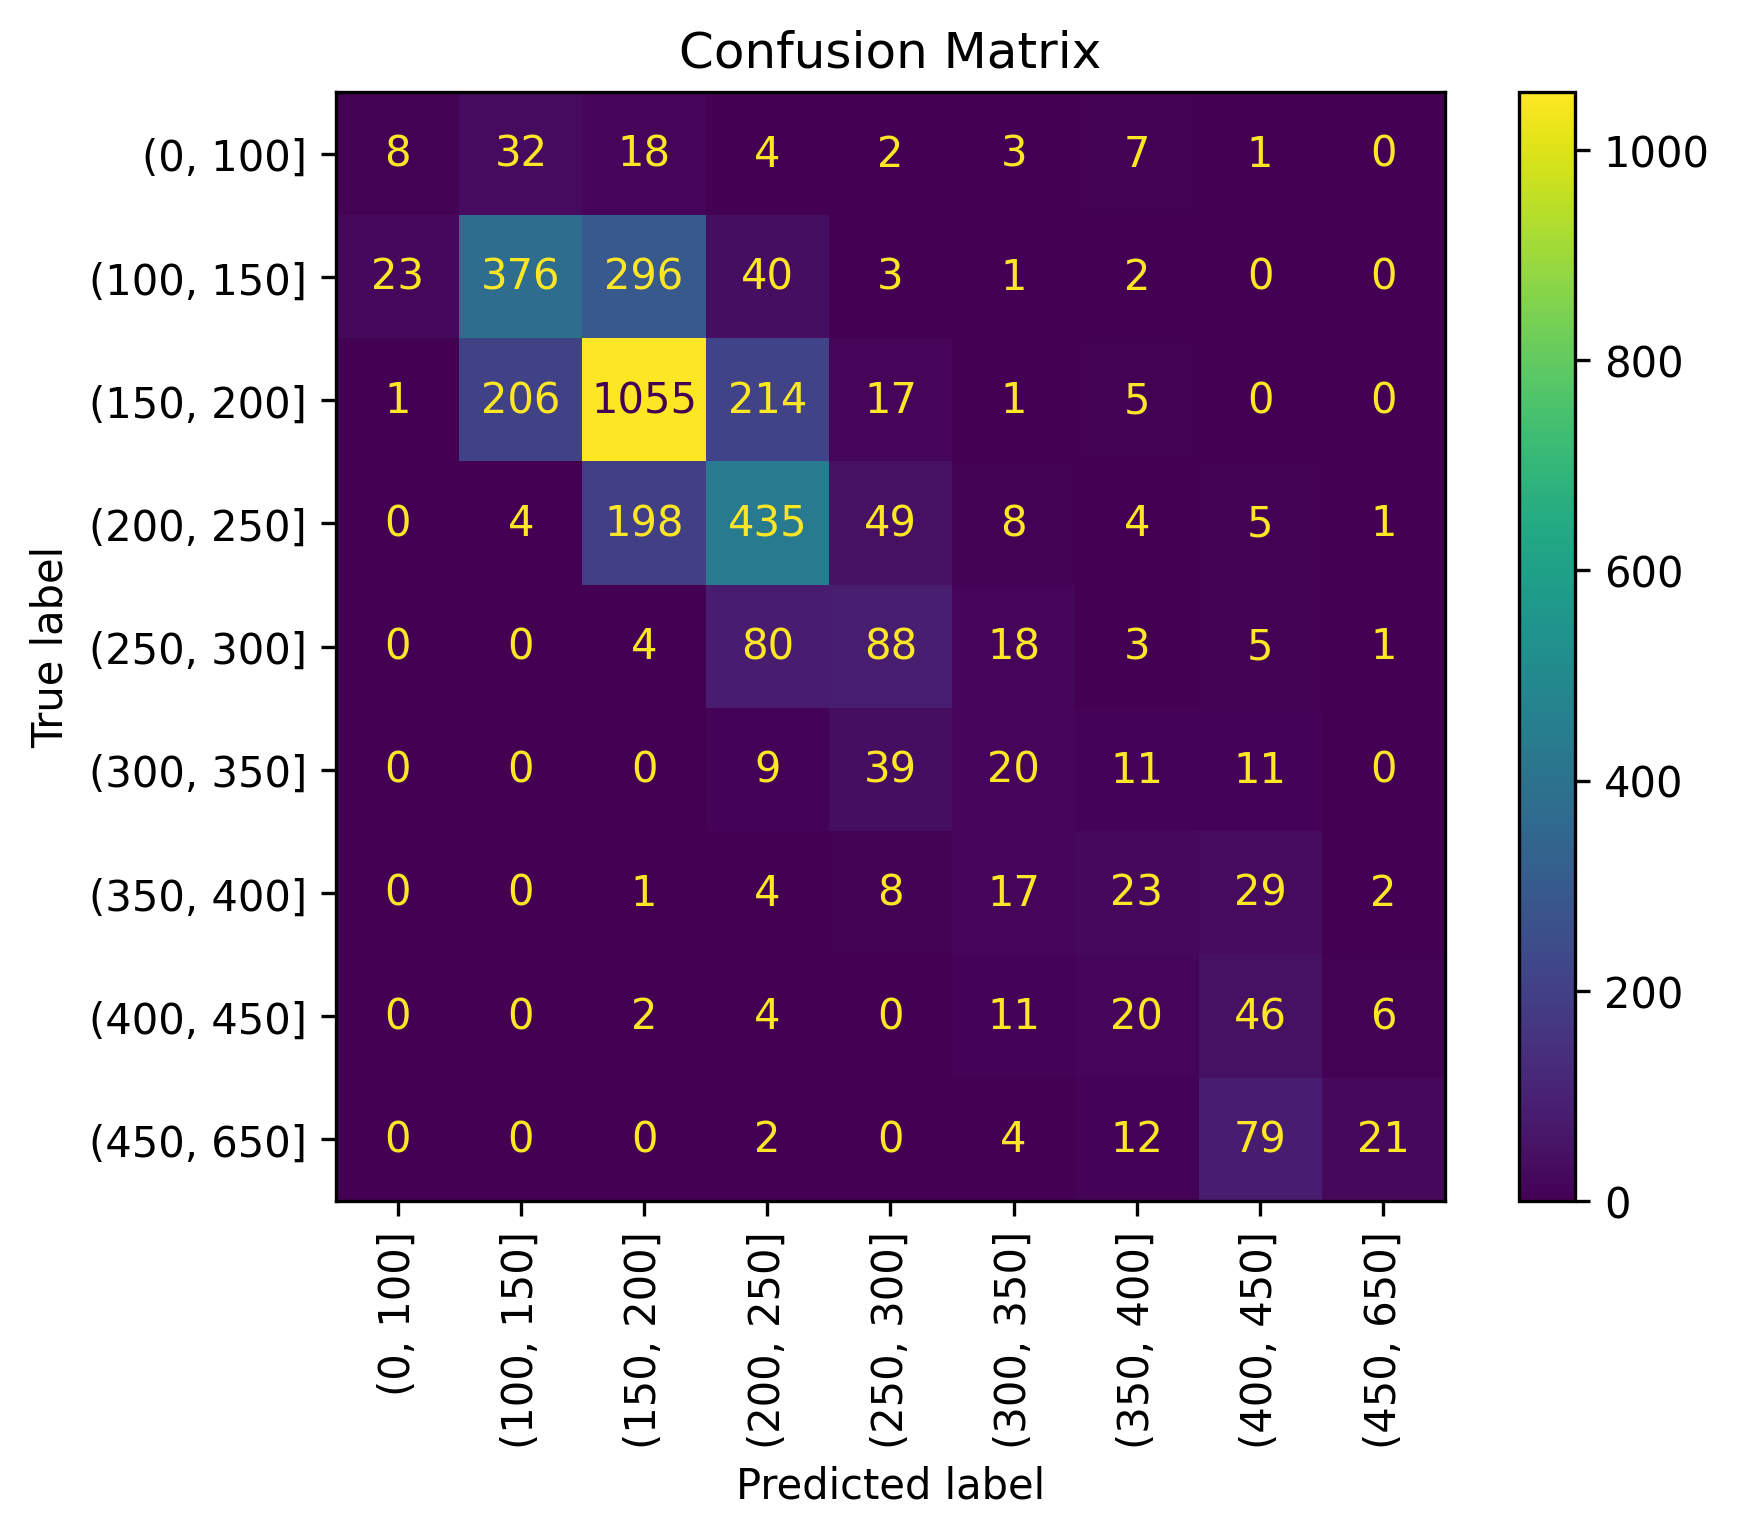
\includegraphics[width=0.9\textwidth]{images/Figure5.png}
    \caption{\textbf{Confusion matrix for linear model fitted by minimizing a regularized empirical loss with stochastic gradient descent.} Aggregated values per bin for observed and predicted values.}\label{fig5}
\end{figure}

The tuned SGD overestimated $paO_2$ values smaller than 100 mmHg and underestimated those larger than 450 mmHg.

We calculated SHAP values to see the contribution of each feature to the prediction, shown in Figure \ref{fig6}. The feature with the highest SHAP value was $pAO_2$, followed by age, and BMI. They were followed by pH value, the respiratory minute volume, temperature values, respiratory compliance, whether or not the patient was mechanically ventilated before entering the operating room and whether or not the observation was made intraoperatively. The remaining 13 features were summed up, as their impact was considered low.

\begin{figure}[h]
    \centering
    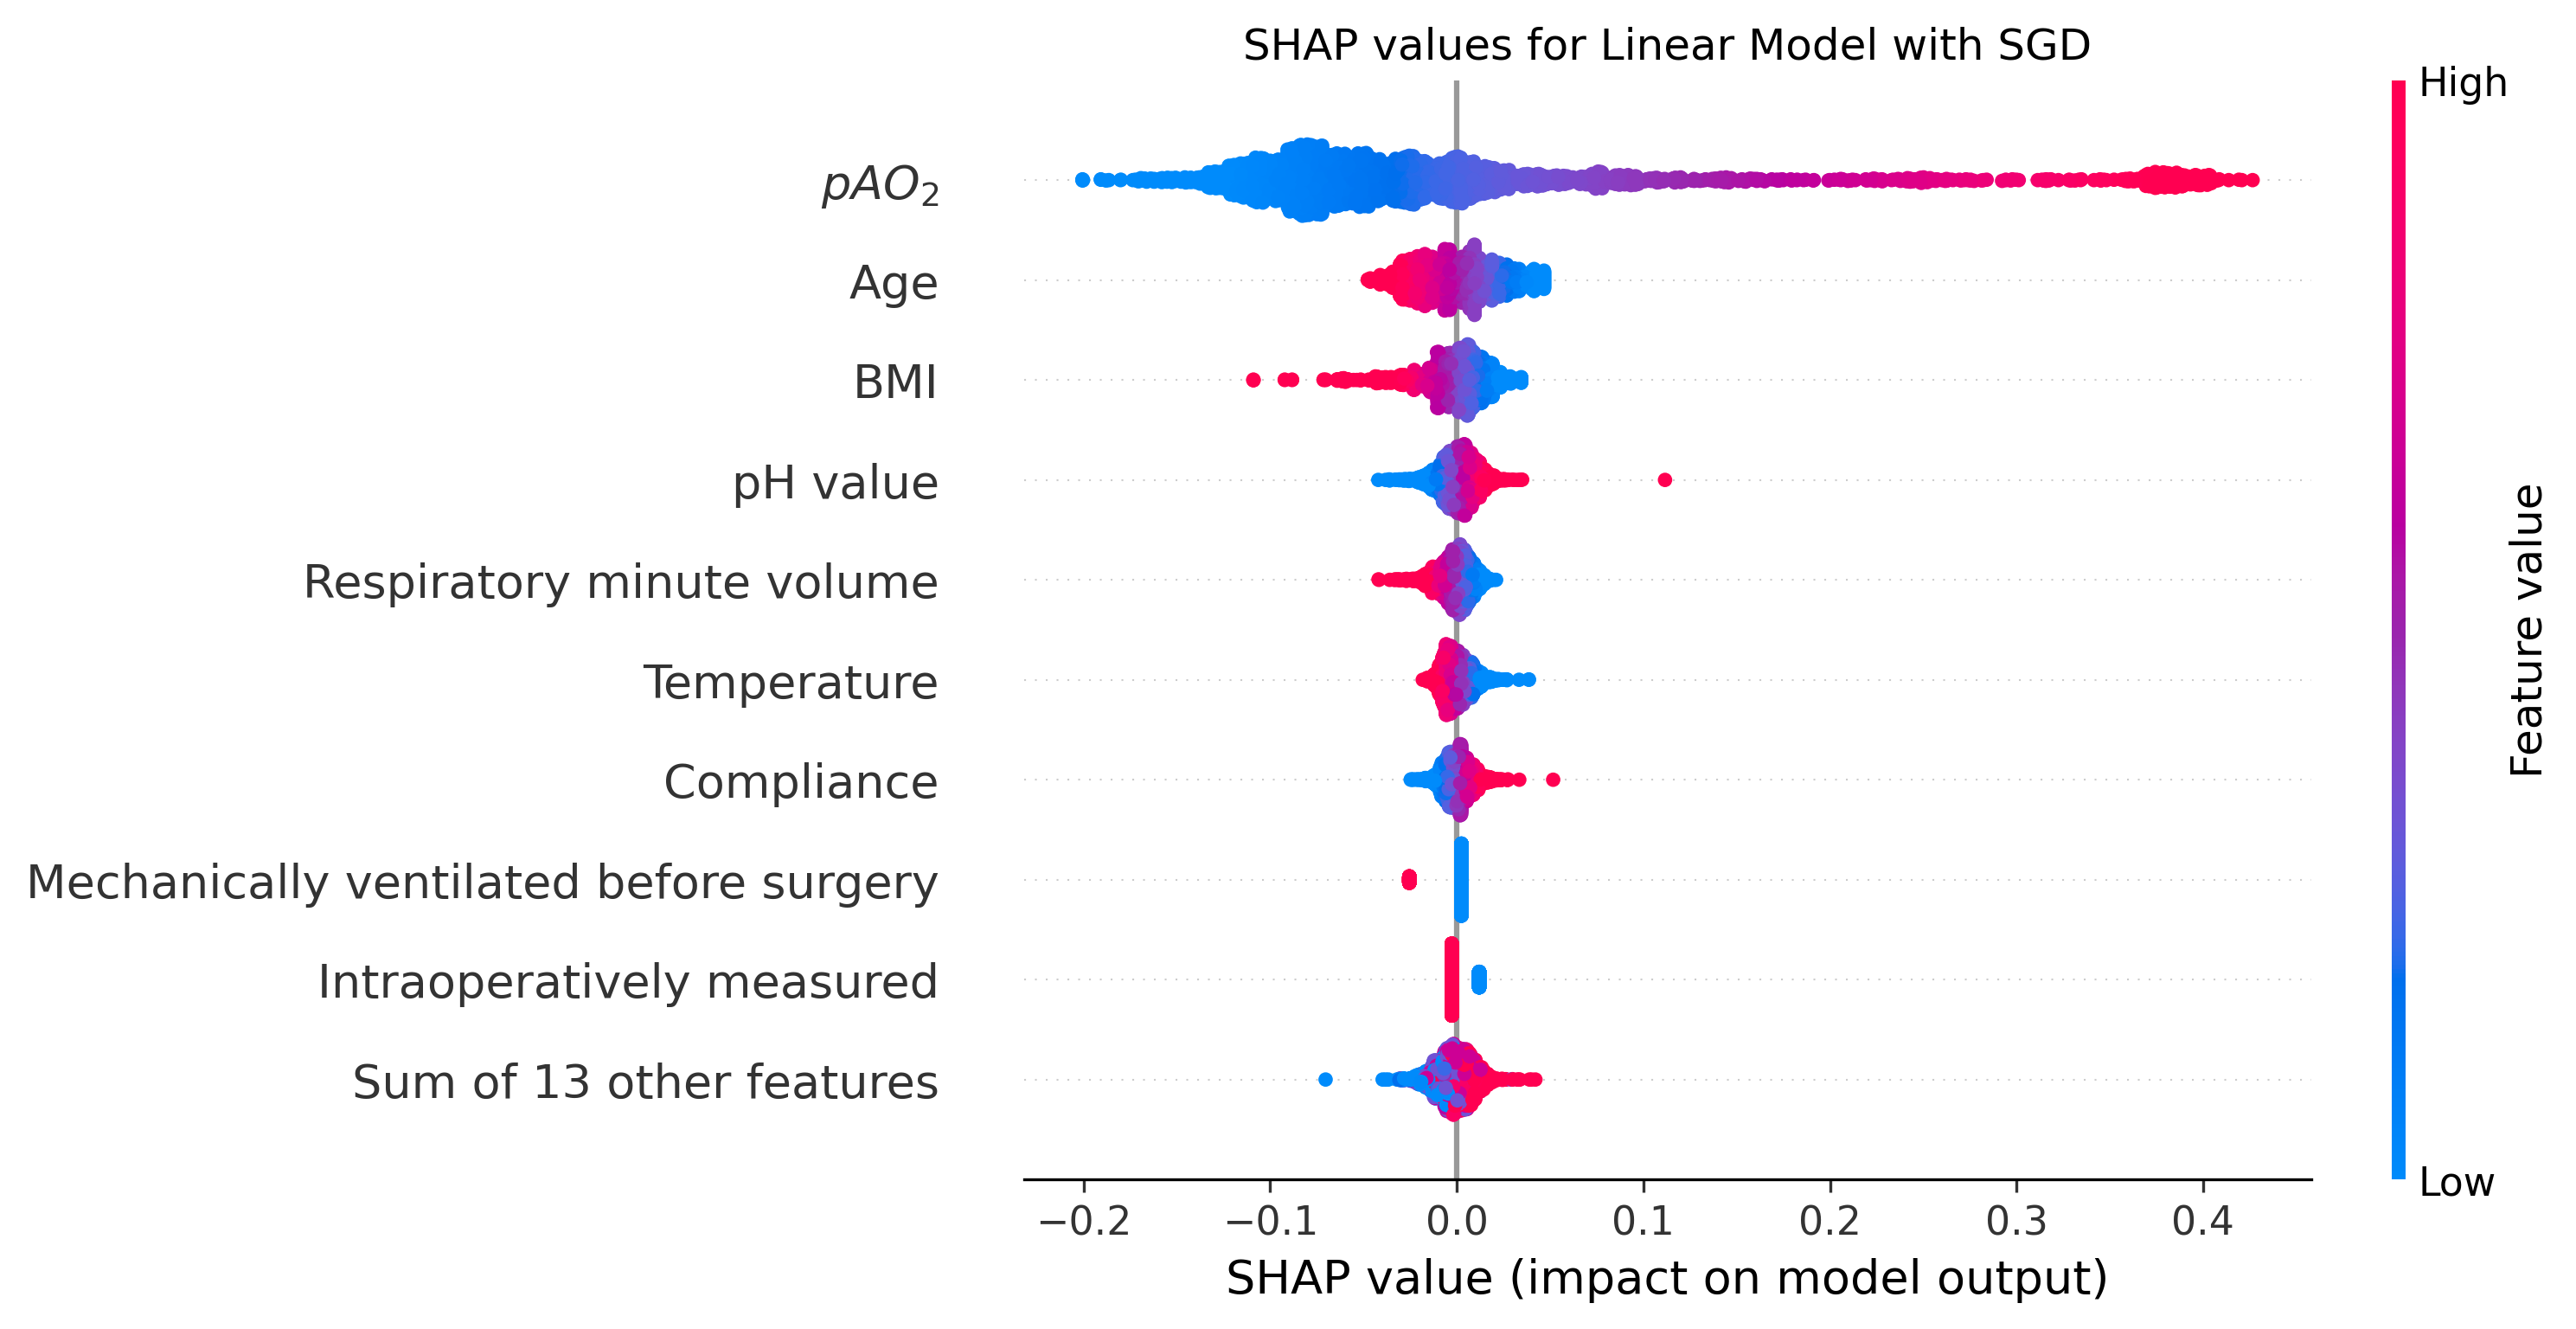
\includegraphics[width=1\linewidth]{images/Figure6.png}
    \caption{\textbf{SHAP values.} Features are ordered by the mean absolute value of the SHAP values.}
    \label{fig6}
\end{figure}

Percentage errors were calculated for all predicted $paO_2$ values; the median was 0.33 \%. Q1 and Q3 were -9.48 \% and 9.28 \%, respectively, resulting in an IQR of 18.75 \%. We investigated all features for the predicted $paO_2$ values that were identified as outliers based on their percentage errors (PE\textless-37.60 \%, PE\textgreater37.40 \%). A total of 237 observations in 133 patients were highly overestimated, 14 observations in 13 patients were highly underestimated (Figure \ref{fig7}). Among those, significant differences were found in three features. 

\begin{figure}[h]
    \centering
    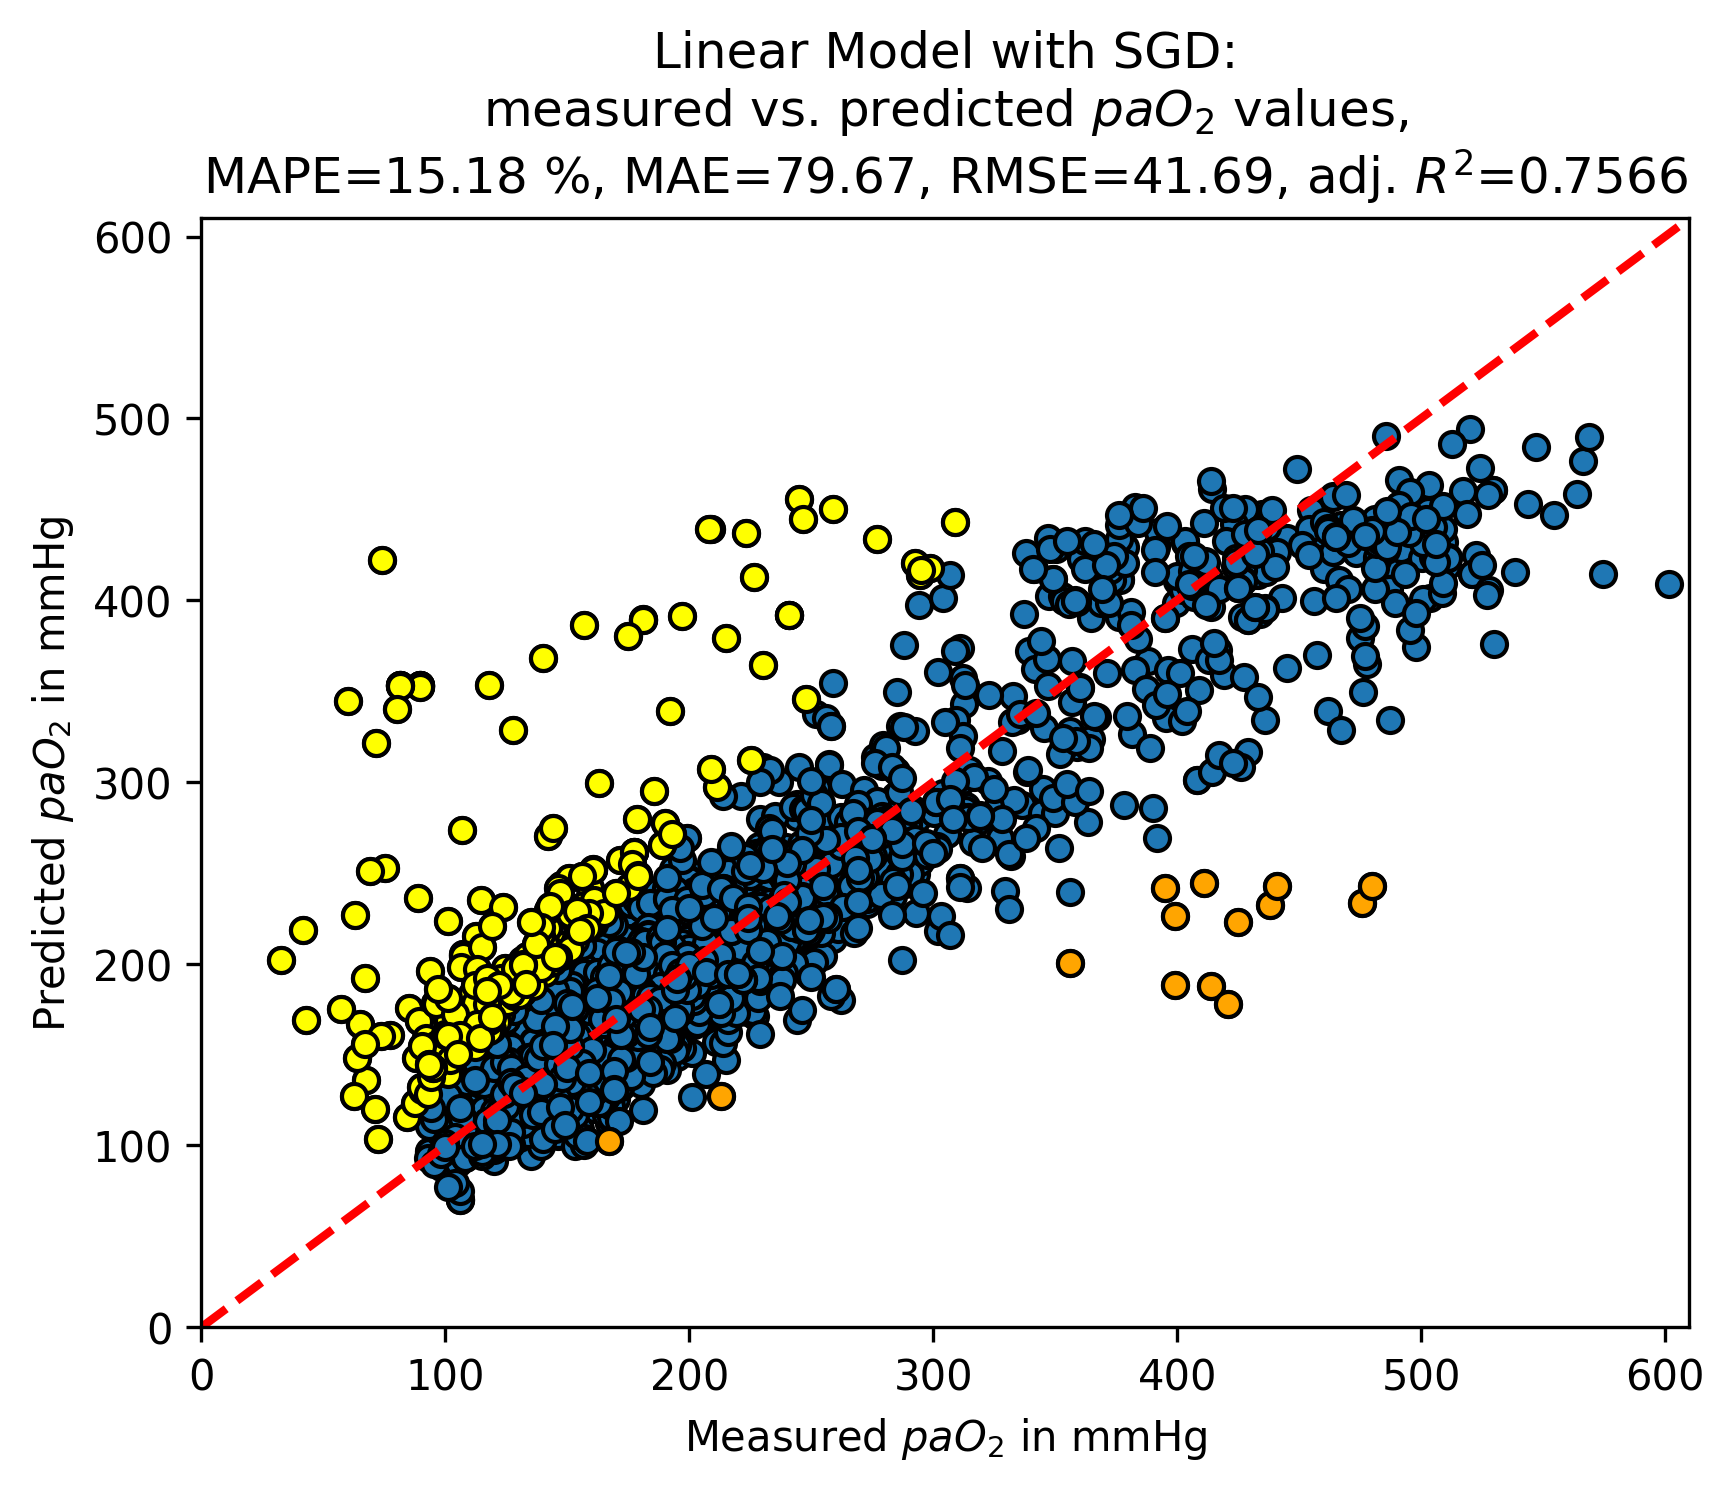
\includegraphics[width=1\linewidth]{images/Figure7.png}
    \caption{\textbf{Evaluation of Linear Model with Stochastic Gradient Descent.} Scatterplot of measured vs. predicted $paO_2$ values with yellow being highly overestimated and orange being highly underestimated values.}
    \label{fig7}
\end{figure}

While most of the underestimated values were based on early observations (between first and second blood sample), overestimated values occurred most often in later observations (between third and fourth measurement). Similar observations were found for the time point of measurement, where 79 \% of the observations in the overestimated group were made intraoperatively, while the observations in the underestimated group were completely balanced (50 \%) between intra- and perioperative. 

The mean temperature in the overestimated observations was 36.2°C, while the mean temperature in the underestimated group was 36.6°C. 


In the last step, we included the first measured p/F ratios in the best model. It improved further: In the test set, the adjusted $R^2$ increased from 0.76 to 0.78, the MAPE decreased by one point to 14.1 \% and the RMSE decreased to 39.3 mmHg. Additionally, the correlation coefficient was now 0.88 [0.87; 0.88], which was significantly better compared to all previously used proxies ($FiO_2$, $pAO_2$, and Gadrey’s $paO_2$). The number of overestimated and underestimated observations could be reduced to 218 and 9, respectively. 

\section{Discussion}\label{sec4}

This study presents a machine learning algorithm for intraoperative live prediction of $paO_2$ values in lung-healthy patients. Although the use of machine learning models in the medical context is not new at all, comparing different algorithms and applying them in a perioperative setting to predict arterial blood gas values is a novel and challenging approach, whose feasibility could be proven with satisfying results. From the selected algorithms, the tuned linear model fitted by minimizing a regularized empirical loss with stochastic gradient descent performed best. Its $paO_2$ predictions were substantially better than the abilities of known proxies or calculation rules to extrapolate on $paO_2$ values. These results allow a closer monitoring of administered oxygen without additional ABGs in lung-healthy patients.

To the best of our knowledge, this is the first study to present a machine learning algorithm for intraoperative live prediction of $paO_2$ values in lung-healthy patients. The continuous assessment of $paO_2$ is currently impossible. Frequent ABGs are time-consuming and potentially harmful for the patient due to the risk of infection and blood loss; in our data, they were collected every 1.9 hours, providing many minutes for additional monitoring with live $paO_2$ predictions. Therefore, $FiO_2$ or $paO_2$ have been used in the past to extrapolate to corresponding $paO_2$ values \cite{Brown2017,Bou-Khalil2017,Sanz2015,Fried1994,Gross1981,Al-Otaibi2011}. In our dataset, the correlation between these values and the actual measured $paO_2$ values was below 0.73, which was considerably worse than the tested algorithms. As $paO_2$ does not directly correlate with the inspiratory fraction of oxygen but $paO_2$ serves as one of the limited tools available to estimate a patient’s degree of hyperoxygenation, we aimed to develop a robust method for estimating perioperative $paO_2$ values based on readily available input parameters. To construct this model, we collected routine data from intracranial neurosurgical operations. These surgeries are particularly well-suited for testing various algorithms for the prediction of intraoperative $paO_2$ for several reasons: First, there is usually an isolated pathology in the neurocranium, and surgical procedures do not impact the thorax, ensuring that gas remains unaffected. Second, arterial catheters are part of the standard monitoring for patients undergoing craniotomy at our clinic. Thirdly, craniotomies typically span three to five hours of surgical time, during which multiple ABGs are drawn, providing a substantial and rich dataset for analysis.

Gadrey et al. were the first to introduce a new equation of $paO_2$ calculation, based on two constant values and the $SpO_2$ value \cite{Gadrey2019}. With $SpO_2$ being the only measured variable, the outcome has a natural maximum of 132.8 mmHg. Thus, the equation is not suitable to model hyperoxemia. Although others used it for predicting arterial partial pressure of oxygen which might only be applicable for a physiological range \cite{Brockway1998,Roettgering2021}. Additionally, the correlation coefficient was relatively low at 0.26 and smaller than the correlation coefficient of $FiO_2$ or $pAO_2$ to the measured $paO_2$ value.


We used machine learning algorithms to model the relatively complex interactions between perioperative and sociodemographic values. The model using a stochastic gradient descent performed best. Two of its main advantages are its computational efficiency and its many options for hyperparameter tuning to fit a specific problem. One of its drawbacks is the sensitivity to feature scaling, requiring all input features to be scaled equally.


\label{limitations}This study faces some limitations. First, our findings are not generalizable to patients with relevant pulmonary dysfunction, such as chronic obstructive pulmonary disease, asthma, lung cancer, or acute respiratory distress syndrome. This cohort was specifically selected to exclude these comorbidities, as our first aim was to investigate which machine learning models would be generally suitable for this task and how well they would perform predictively. Second, besides the surgical procedure and the main diagnosis, we did not consider other comorbidities when training and fitting the different algorithms. The reason for this was the need to develop a generalizable algorithm, which could be used in a broad range of patients with different kinds of comorbidities but the same type of surgical procedure. Still, with MAPEs of 15 \% and 14 \% (when including the first measured p/F ratio), our algorithm yielded very accurate results. Third, we only included patients with invasive ventilation and general anesthesia who received at least two ABGs. Fourth, in the range of hypoxic and normoxic $paO_2$ values (up to 100 mmHg), we rather overestimate the $paO_2$ value, whereas in severe hyperoxia (more than 450 mmHg) we rather underestimate the true value (Figure \ref{fig7}). Sixth, the study size might be too small for deep learning methods to deploy their full potential \cite{Benkendorf2020,Liu2017}. 

\section{Conclusion}\label{sec5}
In this study, we demonstrate that machine learning algorithms can be utilized to predict $paO_2$ values for a range between 100 to 450 mmHg. Our SGD did not only achieve the highest adjusted $R2$ of 0.76 and 0.78 (when including the first measured p/F ratio), the lowest MAPE of 15 \%, but also the highest correlation coefficient and the smallest RMSE. Although some papers exist that extrapolate $paO_2$ values, this is the first model for live prediction of $paO_2$ values with satisfactory results. Such a tool might support medical staff to continuously estimate $paO_2$ values to enhance monitoring and prevention of hyperoxemia in a perioperative setting. Continuous in-silico prediction of $paO_2$ levels might also enhance estimation of the total excess of oxygen during patient treatment, allowing researchers to better investigate its effects.

Our next study will use these results for a quasi-real time prediction in the same patient collective to evaluate the effect of excessive oxygen on postoperative complications. Besides that, future studies are needed to validate our method in other patient collectives and clinical scenarios. 

%\end{linenumbers}

\section*{Declarations}

\subsection*{Funding}\label{funding}
The study received no funding.

\subsection*{Conflict of interest/Competing interests}
All authors declare no financial or non-financial competing interests.

\subsection*{Ethics approval and consent to participate}
The study was conducted as a single-center retrospective cohort study.  Before accessing the data, our protocol (submission 19-539) received approval from the University of Munich’s institutional review board. The requirement for informed consent was waived from the Ethics Committee of University of Munich’s institutional review board because of the retrospective nature of the study.

\subsection*{Consent for publication}

\subsection*{Data and Code availability}
The code and rendered notebook files supporting the conclusion of this article are publicly available in the git repository: \href{https://github.com/abeckerp/pao2-prediction}{https://github.com/abeckerp/pao2-prediction}.

\subsection*{Author contribution}
\textbf{CRediT author statement}
Andrea S Gutmann: Methodology, Software, Formal Analysis, Data Curation, Writing - Original Draft, Visualization, Investigation\\
Maximilian M Mandl: Methodology, Validation, Writing - Review \& Editing\\
Clemens Rieder: Writing - Review \& Editing\\
Dominik J Hoechter: Writing - Review \& Editing\\
Konstantin Dietz: Writing - Review \& Editing\\
Benjamin P Geisler: Writing - Review \& Editing\\
Anne-Laure Boulesteix: Conceptualization, Validation, Supervision, Writing - Review \& Editing\\
Roland Tomasi: Validation, Resources, Writing - Review \& Editing\\
Ludwig C Hinske: Conceptualization, Resources, Writing - Review \& Editing, Supervision


\bibliography{references}

\begin{appendices}\label{appendices}

\section{Formulas used for Features}\label{secA1}
\begin{itemize}
\item Alveolar gas equation: $pAO_2=\frac{FiO_2}{100} * (713.622 - 47) - \frac{CO_2}{0.82}$, assuming a prevailing atmospheric pressure of 713.622 mmHg and a saturated vapor pressure of water of 47 mmHg \cite{Sharma2019}
\item Static compliance: $C_{stat}=\frac{RMV}{RR}*\frac{1000}{P_{plat}-PEEP}=\frac{V}{P_{plat}-PEEP},\;where\;V=\frac{RMV}{RR}*1000$ with $RMV$ as the respiratory minute volume, $RR$ as the respiratory rate, $P_{plat}$ as the plateau pressure in cm $H_20$ and $PEEP$ as the positive end-expiratory pressure in cm $H_20$ \cite{Desai2019}
\item $Gadrey's paO_2=\frac{23400}{\frac{1}{SpO_2}-0.99}^{\frac{1}{3}}$ \cite{Gadrey2019}
\item Feature and label scaling based on training data using the min-max normalization: $x_{scaled}=s*(max-min)+min,\;with\;s=(x-x_{min})/(x_{max}-x_{min})\;and\;min=0,\;max=1$ \cite{Pedregosa2011, Han2012}
\end{itemize}

\section{List of Features}\label{secA2}
Full list of features:
\begin{itemize}
    \item identifier: identifier for surgery,
    \item idx: incrementing number of the measurement (discrete value),
    \item fio2: inspiratory fraction of oxygen (continuous value), 
    \item co2: end-tidal carbon dioxide in mmHg (continuous value), 
    \item spo2: peripheral capillary oxygen saturation in \% (continuous value),
    \item rmv: respiratory minute volume in liter (continuous value), 
    \item respiratory\_rate: respiratory rate in 1/minute (discrete value), 
    \item compliance: ventilation compliance in milliliter\/millibar (continuous value), 
    \item paO2\_measured: measured $paO_2$ value in mmHg (continuous value),
    \item first\_horowitz: first $paO_2/FiO_2$ ratio in mmHg (continuous value), 
    \item last\_horowitz: last measured $paO_2/FiO_2$ ratio in mmHg (continuous value),
    \item pAO2: $pAO_2$ calculated value by the alveolar gas equation in mmHg (continuous value), 
    \item systolic: systolic value in mmHg (discrete value), 
    \item diastolic: diastolic value in mmHg (discrete value), 
    \item mean\_art\_press: mean arterial pressure in mmHg (discrete value), 
    \item heart\_rate: heart rate in 1/minute (discrete value), 
    \item temperature: temperature value in degree celsius (continuous value),
    \item ph: last measured pH-value (different sampling sites) (continuous value), 
    \item hemoglobin: last measured hemoglobin value in g\/dL (different sampling sites) (continuous value), 
    \item case\_number: a patient’s case number during a hospital stay
    \item already\_intubated: indicates whether a patient was already intubated before surgery (dichotomous value),
    \item not\_extubated: indicates whether a patient was not extubated after surgery (dichotomous value),
    \item bmi: a patient’s body mass index (continuous value),
    \item age: age in years (continuous value), 
    \item los: postoperative length-of-stay in days (continuous value),
    \item creatinine: pre-operative creatinine value in milligram\/deciliter (continuous value), 
    \item time\_to\_incision: time from intubation to incision in minutes (continuous value),
    \item time\_to\_end: time from suture to extubation in minutes (continuous value),
    \item mv\_time: invasive mechanical ventilation time in minutes (continuous value),
    \item incision\_closure\_time: time in minutes from incision to closure (continuous value),
    \item gadrey: paO2 values calculated by Gadrey et al. in mmHg [30] (continuous value),
    \item sex\_male: indicates a male patient (dichotomous value),
    \item asa: patient’s ASA score (discrete value),
    \item timepoint\_intraop: indicates whether the measurement was done intraoperatively (dichotomous value)
\end{itemize}

Features not eligible for recursive feature elimination, hyperparameter tuning and evaluation:
\begin{itemize}
\item paO2\_measured,
\item los
\item identifier,
\item incision\_closure\_time,
\item mv\_time,
\item time\_to\_incision,
\item time\_to\_end,
\item not\_extubated,
\item first\_horowitz,
\item last\_horowitz,
\item case\_number
\end{itemize}

\section{Inclusion and Exclusion Criteria}\label{secA3}
Observations with negative $paO_2$ values were excluded. Then, surgeries with invalid parameters were excluded; those were missing or negative data on postoperative length-of-stay, missing or measured creatinine values of \textless0.2 mg/dL, a BMI \textless14 or \textgreater60 kg/m\textsuperscript{2}, an initial intraoperative p/F ratio \textless300 mmHg (indicating impaired lung oxygenation), and surgeries with less than 5 min incision-to-closure time or mechanical ventilation times and negative times to incision or to end. Secondly, observations with negative ABG values or missing $FiO_2$, $CO_2$, or $SpO_2$ were excluded. Additional exclusion criteria consisted of measured hemoglobin levels \textless5 g/dL \cite{ref5,Lundsgaard-Hansen1989}, recorded blood pH values \textless6.8, a heart rate <20/min, a respiratory rate \textless5/min, a respiratory minute volume \textless2 l/min. We also removed observations with body temperature measurements \textless32°C, which we interpreted as a disconnected temperature sensor. Additionally, observations with measured $paO_2$ values \textless60 mmHg were excluded if hemoglobin values exceeded 7 g/dL and $SpO_2$ levels exceeded 95 \%, as these values were likely attributed to venous blood gas analysis rather than arterial (Figure \ref{fig8}).

\begin{figure}[h]
    \centering
    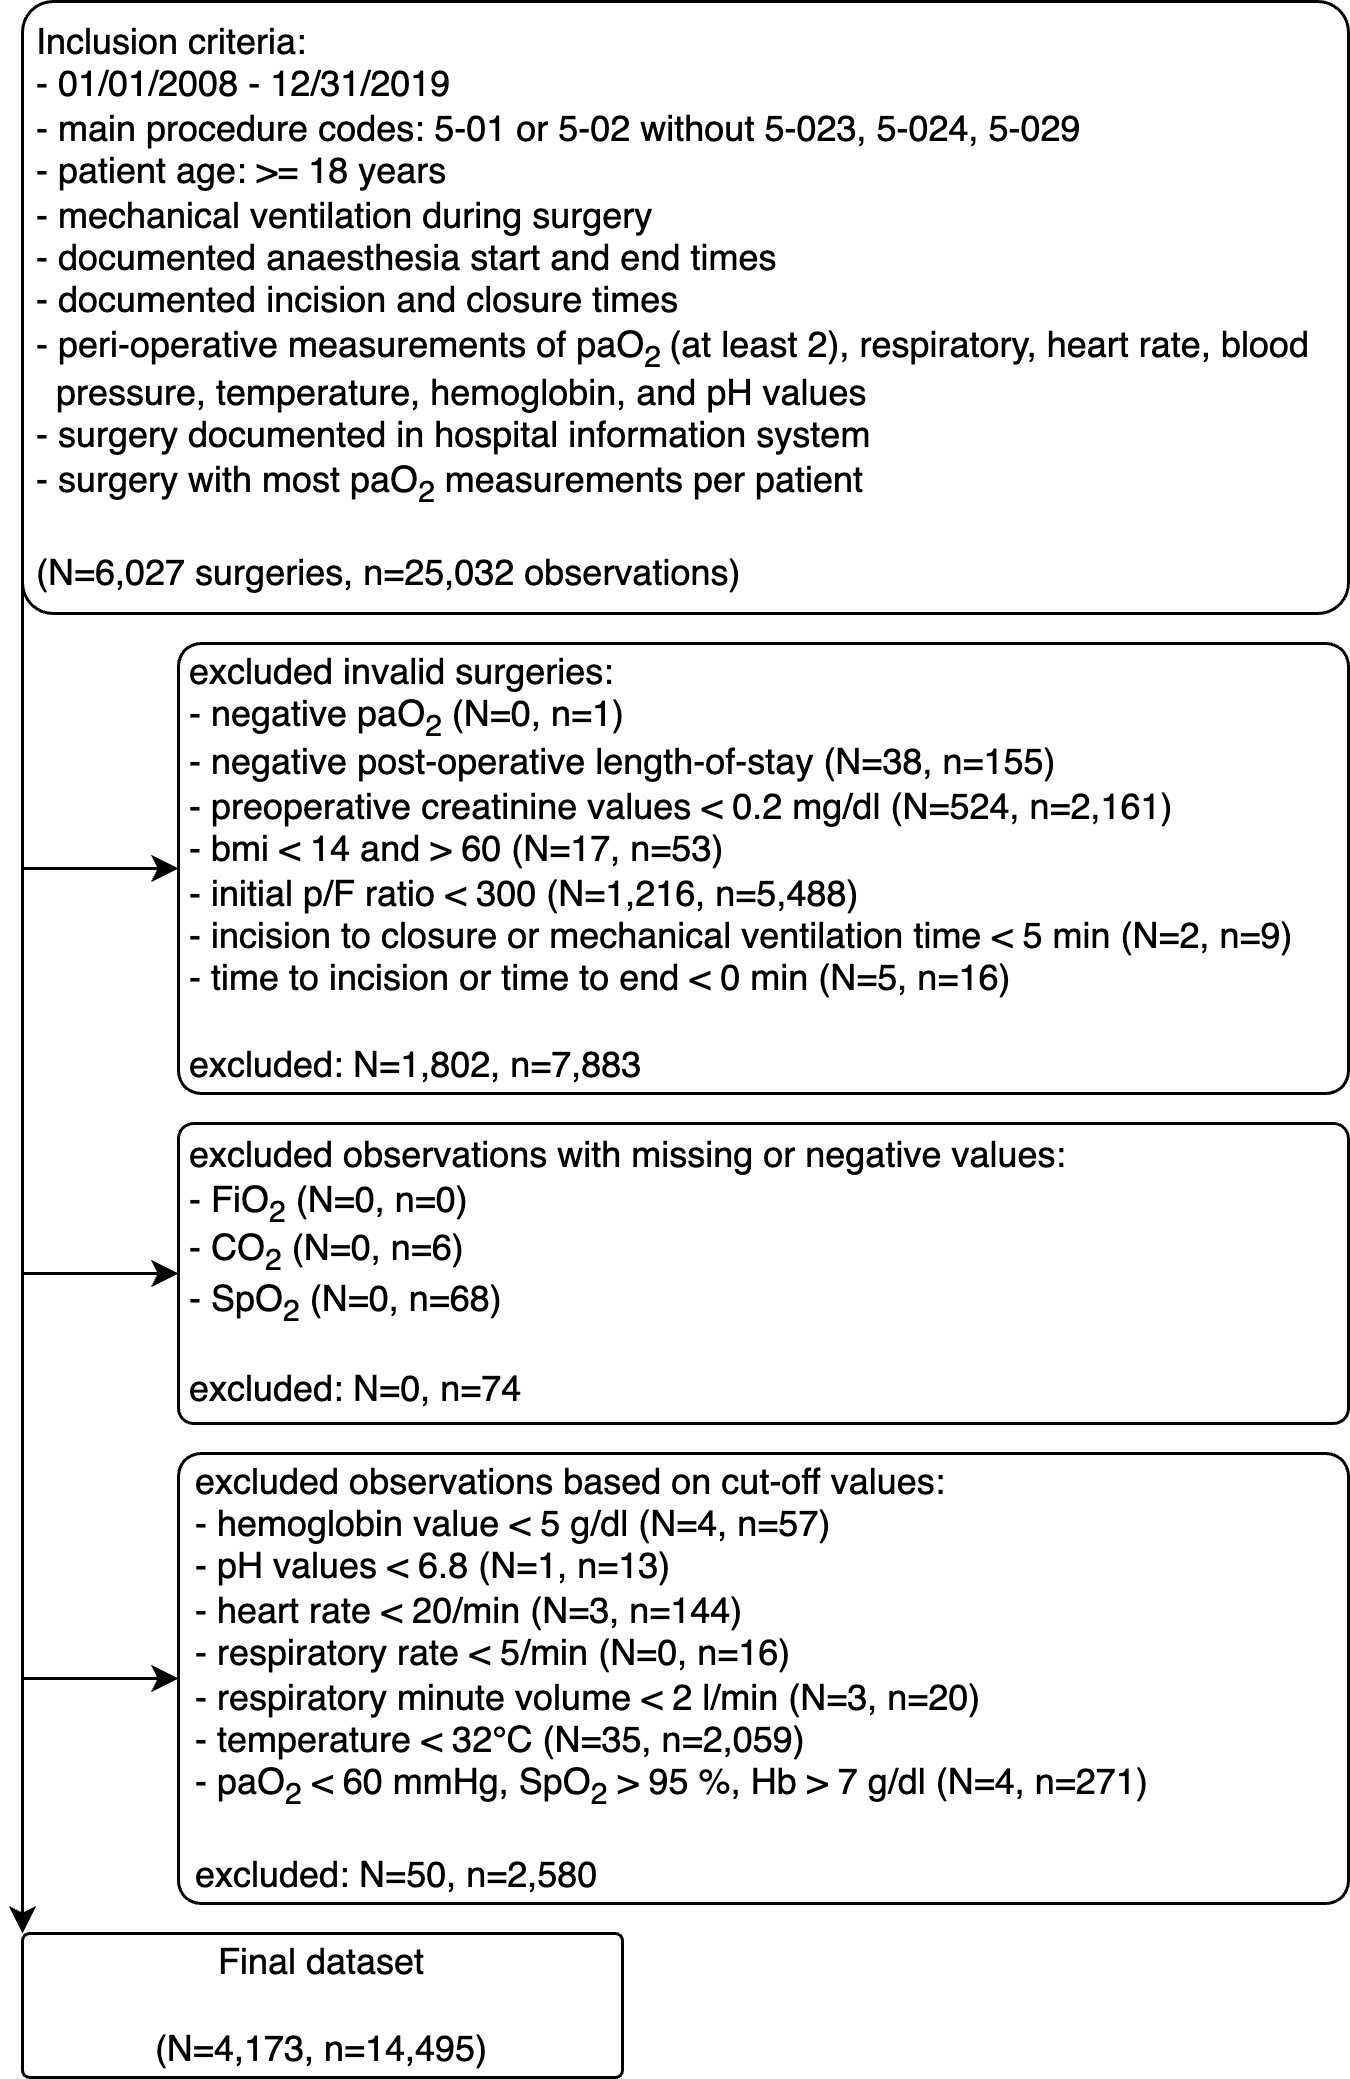
\includegraphics[width=1\linewidth]{images/Figure8.png}
    \caption{\textbf{Patient flowchart with inclusion and exclusion criteria.} }
    \label{fig8}
\end{figure}

\section{Default and Final Parameters of Estimators}\label{secA4}

\subsection{Gradient Boosting for Regression}\label{secA4.1}

\begin{table}[h]
    \caption{Gradient Boosting for Regression}%
    \begin{tabular}{@{}llll@{}}
        \toprule
        & Default Parameters & Hyperparameters & Best Parameters \\
        \midrule
        alpha & 0.900000 & & 0.900000 \\
        ccp\_alpha & 0.000000 & & 0.000000 \\
        criterion & friedman\_mse & & friedman\_mse \\
        init & & & None \\
        learning\_rate & 0.100000 & {[}0.01 0.2075 0.405 0.6025 0.8 {]} &
        0.207500 \\
        loss & squared\_error &
        {[}\textquotesingle squared\_error\textquotesingle,
        \textquotesingle huber\textquotesingle,
        \textquotesingle quantile\textquotesingle{]} & squared\_error \\
        max\_depth & 3 & {[}2, 3, 4, 5, 6, None{]} & 2 \\
        max\_features & & & None \\
        max\_leaf\_nodes & & & None \\
        min\_impurity\_decrease & 0.000000 & & 0.000000 \\
        min\_samples\_leaf & 1 & {[}1, 2, 3, 4{]} & 3 \\
        min\_samples\_split & 2 & & 2 \\
        min\_weight\_fraction\_leaf & 0.000000 & & 0.000000 \\
        n\_estimators & 100 & {[}50, 80, 100, 120, 150{]} & 50 \\
        n\_iter\_no\_change & & & None \\
        random\_state & 42 & & 42 \\
        subsample & 1.000000 & & 1.000000 \\
        tol & 0.000100 & & 0.000100 \\
        validation\_fraction & 0.100000 & & 0.100000 \\
        verbose & 0 & & 0 \\
        warm\_start & False & & False \\
        \botrule
    \end{tabular}
    \footnotetext{Default, hyper- and best parameters.}
\end{table}

\subsection{K-nearest Neighbors Regression}\label{secA4.2}

\begin{table}[h]
    \caption{K-nearest Neighbors Regression}%
    \begin{tabular}{@{}llll@{}}
        \toprule
        & Default Parameters & Hyperparameters & Best Parameters \\
        \midrule
        algorithm & auto & {[}\textquotesingle ball\_tree\textquotesingle,
        \textquotesingle kd\_tree\textquotesingle,
        \textquotesingle brute\textquotesingle,
        \textquotesingle auto\textquotesingle{]} & ball\_tree \\
        leaf\_size & 30 & {[} 5 10 15 20 25 30 35 40 45 50{]} & 15 \\
        metric & minkowski & {[}\textquotesingle minkowski\textquotesingle,
        \textquotesingle l1\textquotesingle,
        \textquotesingle l2\textquotesingle{]} & minkowski \\
        metric\_params & & & None \\
        n\_jobs & & & None \\
        n\_neighbors & 5 & {[} 5 13 21 29 37 45{]} & 21 \\
        p & 2 & {[}1, 2{]} & 1 \\
        weights & uniform & {[}\textquotesingle uniform\textquotesingle,
        \textquotesingle distance\textquotesingle{]} & uniform \\
        \botrule
    \end{tabular}
    \footnotetext{Default, hyper- and best parameters.}
\end{table}



\subsection{Random Forest Regressor}\label{secA4.3}

\begin{table}[h]
    \caption{Random Forest Regressor}%
    \begin{tabular}{@{}llll@{}}
        \toprule
        & Default Parameters & Hyperparameters & Best Parameters \\
        \midrule
        bootstrap & True & {[}True{]} & True \\
        ccp\_alpha & 0.000000 & & 0.000000 \\
        criterion & squared\_error &
        {[}\textquotesingle squared\_error\textquotesingle,
        \textquotesingle friedman\_mse\textquotesingle{]} & friedman\_mse \\
        max\_depth & & {[}3, 9, 16, 23, 30{]} & 9 \\
        max\_features & 1.000000 & {[}\textquotesingle sqrt\textquotesingle,
        \textquotesingle log2\textquotesingle, 0.6, 1.0{]} & log2 \\
        max\_leaf\_nodes & & & None \\
        max\_samples & & & None \\
        min\_impurity\_decrease & 0.000000 & & 0.000000 \\
        min\_samples\_leaf & 1 & {[}1 4 7{]} & 1 \\
        min\_samples\_split & 2 & {[}2, 4, 6{]} & 4 \\
        min\_weight\_fraction\_leaf & 0.000000 & & 0.000000 \\
        n\_estimators & 100 & {[}50, 87, 125, 162, 200{]} & 200 \\
        n\_jobs & & & None \\
        oob\_score & False & & False \\
        random\_state & 42 & & 42 \\
        verbose & 0 & & 0 \\
        warm\_start & False & & False \\
        \botrule
    \end{tabular}
    \footnotetext{Default, hyper- and best parameters.}
\end{table}


\subsection{Epsilon-Support Vector Regression}\label{secA4.4}

\begin{table}[h]
    \caption{Epsilon-Support Vector Regression}%
    \begin{tabular}{@{}llll@{}}
        \toprule
        & Default Parameters & Hyperparameters & Best Parameters \\
        \midrule
        C & 1.000000 & {[}0.01, 0.1, 1.0, 10, 100{]} & 0.100000 \\
        cache\_size & 200 & {[}10000{]} & 10000 \\
        coef0 & 0.000000 & {[}0.0, 0.1, 0.2{]} & 0.100000 \\
        degree & 3 & & 3 \\
        epsilon & 0.100000 & {[}0.001, 0.01, 0.1, 1.0, 10{]} & 0.100000 \\
        gamma & scale & {[}\textquotesingle auto\textquotesingle,
        \textquotesingle scale\textquotesingle{]} & scale \\
        kernel & rbf & {[}\textquotesingle rbf\textquotesingle,
        \textquotesingle sigmoid\textquotesingle{]} & rbf \\
        max\_iter & -1 & & -1 \\
        shrinking & True & {[}True, False{]} & False \\
        tol & 0.001000 & {[}0.0001, 0.001, 0.01, 0.1, 1.0{]} & 0.010000 \\
        verbose & False & & False \\
        \botrule
    \end{tabular}
    \footnotetext{Default, hyper- and best parameters.}
\end{table}


\subsection{Linear model with SGD}\label{secA4.5}

\begin{sidewaystable}
    \caption{Linear model fitted by minimizing a regularized empirical loss with stochastic gradient descent}%
    \begin{tabularx}{\textwidth}{@{} l l LLLLL @{}}
    % \begin{tabular}{@{}lllllll@{}}
        \toprule
        & Default Parameters & Hyperparameters1 & Hyperparameters2 & Hyperparameters3 & Hyperparameters4 & Best Parameters \\
        \midrule
        alpha & 0.000100 & {[}1e-05, 0.0001, 0.001, 0.01, 0.1{]} & {[}1e-05,
        0.0001, 0.001, 0.01, 0.1{]} & {[}1e-05, 0.0001, 0.001, 0.01, 0.1{]} &
        {[}1e-05, 0.0001, 0.001, 0.01, 0.1{]} & 0.000010 \\
        average & False & & & & & False \\
        early\_stopping & False & & & & & False \\
        epsilon & 0.100000 & {[}0.01, 0.1, 0.5{]} & {[}0.01, 0.1, 0.5{]} &
        {[}0.01, 0.1, 0.5{]} & {[}0.01, 0.1, 0.5{]} & 0.500000 \\
        eta0 & 0.010000 & {[}0.001, 0.01, 0.1{]} & {[}0.001, 0.01, 0.1{]} &
        {[}0.001, 0.01, 0.1{]} & {[}0.001, 0.01, 0.1{]} & 0.100000 \\
        fit\_intercept & True & & & & & True \\
        l1\_ratio & 0.150000 & & & {[}0.1, 0.15, 0.2, 0.5{]} & {[}0.1, 0.15,
        0.2, 0.5{]} & 0.500000 \\
        learning\_rate & invscaling &
        {[}\textquotesingle constant\textquotesingle,
        \textquotesingle optimal\textquotesingle,
        \textquotesingle invscaling\textquotesingle,
        \textquotesingle adaptive\textquotesingle{]} &
        {[}\textquotesingle constant\textquotesingle,
        \textquotesingle optimal\textquotesingle,
        \textquotesingle invscaling\textquotesingle,
        \textquotesingle adaptive\textquotesingle{]} &
        {[}\textquotesingle constant\textquotesingle,
        \textquotesingle optimal\textquotesingle,
        \textquotesingle invscaling\textquotesingle,
        \textquotesingle adaptive\textquotesingle{]} &
        {[}\textquotesingle constant\textquotesingle,
        \textquotesingle optimal\textquotesingle,
        \textquotesingle invscaling\textquotesingle,
        \textquotesingle adaptive\textquotesingle{]} & adaptive \\
        loss & squared\_error &
        {[}\textquotesingle squared\_error\textquotesingle{]} &
        {[}\textquotesingle epsilon\_insensitive\textquotesingle,
        \textquotesingle squared\_epsilon\_insensitive\textquotesingle{]} &
        {[}\textquotesingle squared\_error\textquotesingle{]} &
        {[}\textquotesingle epsilon\_insensitive\textquotesingle,
        \textquotesingle squared\_epsilon\_insensitive\textquotesingle{]} &
        squared\_error \\
        max\_iter & 100000000 & & & & & 100000000 \\
        n\_iter\_no\_change & 5 & & & & & 5 \\
        penalty & l2 & {[}None, \textquotesingle l2\textquotesingle,
        \textquotesingle l1\textquotesingle{]} & {[}None,
        \textquotesingle l2\textquotesingle,
        \textquotesingle l1\textquotesingle{]} &
        {[}\textquotesingle elasticnet\textquotesingle{]} &
        {[}\textquotesingle elasticnet\textquotesingle{]} & elasticnet \\
        power\_t & 0.250000 & {[}0.1, 0.25, 0.5, 0.7{]} & {[}0.1, 0.25, 0.5,
        0.7{]} & {[}0.1, 0.25, 0.5, 0.7{]} & {[}0.1, 0.25, 0.5, 0.7{]} &
        0.100000 \\
        random\_state & 42 & & & & & 42 \\
        shuffle & True & & & & & True \\
        tol & 0.001000 & {[}0.0001, 0.001, 0.01, 0.1{]} & {[}0.0001, 0.001,
        0.01, 0.1{]} & {[}0.0001, 0.001, 0.01, 0.1{]} & {[}0.0001, 0.001, 0.01,
        0.1{]} & 0.001000 \\
        validation\_fraction & 0.100000 & & & & & 0.100000 \\
        verbose & 0 & & & & & 0 \\
        warm\_start & False & & & & & False \\
        \botrule
    % \end{tabular}
    \end{tabularx}
    \footnotetext{Default, hyper- and best parameters.}
\end{sidewaystable}


\subsection{Multivariable ordinary least squares Linear Regression}\label{secA4.6}

\begin{table}[h]
    \caption{Multivariable ordinary least squares Linear Regression}%
    \begin{tabular}{@{}llll@{}}
        \toprule
        & Default Parameters & Hyperparameters & Best Parameters \\
        \midrule
        copy\_X & True & {[}False, True{]} & False \\
        fit\_intercept & True & {[}False, True{]} & True \\
        n\_jobs & & & None \\
        positive & False & {[}False, True{]} & True \\
        \botrule
    \end{tabular}
    \footnotetext{Default, hyper- and best parameters.}
\end{table}

\subsection{Multi-layer Perceptron Regressor}\label{secA4.7}

\begin{sidewaystable}
    \caption{Multi-layer Perceptron Regressor}%
    \begin{tabularx}{\textwidth}{@{} l l LLLLL @{}}
        \toprule
        & Default Parameters & Hyperparameters1 & Hyperparameters2 & Hyperparameters3 & Hyperparameters4 & Best Parameters \\
        \midrule
        activation & relu & {[}\textquotesingle relu\textquotesingle,
        \textquotesingle tanh\textquotesingle,
        \textquotesingle logistic\textquotesingle{]} &
        {[}\textquotesingle relu\textquotesingle,
        \textquotesingle tanh\textquotesingle,
        \textquotesingle logistic\textquotesingle{]} &
        {[}\textquotesingle relu\textquotesingle,
        \textquotesingle tanh\textquotesingle,
        \textquotesingle logistic\textquotesingle{]} &
        {[}\textquotesingle relu\textquotesingle,
        \textquotesingle tanh\textquotesingle,
        \textquotesingle logistic\textquotesingle{]} & tanh \\
        alpha & 0.000100 & {[}0.0001, 0.001{]} & {[}0.0001, 0.001{]} &
        {[}0.0001, 0.001{]} & {[}0.0001, 0.001{]} & 0.000100 \\
        batch\_size & auto & {[}\textquotesingle auto\textquotesingle, 64,
        128{]} & {[}\textquotesingle auto\textquotesingle, 64, 128{]} &
        {[}\textquotesingle auto\textquotesingle, 64, 128{]} &
        {[}\textquotesingle auto\textquotesingle, 64, 128{]} & 128 \\
        beta\_1 & 0.900000 & & & & & 0.900000 \\
        beta\_2 & 0.999000 & & & & & 0.999000 \\
        early\_stopping & False & {[}True{]} & {[}True{]} & {[}True{]} &
        {[}True{]} & True \\
        epsilon & 0.000000 & & & & & 0.000000 \\
        hidden\_layer\_sizes & (100,) & {[}(100,), (256, 128), (64,), (256, 128,
        64), (64, 32){]} & {[}(100,), (256, 128), (64,), (256, 128, 64), (64,
        32){]} & {[}(100,), (256, 128), (64,), (256, 128, 64), (64, 32){]} &
        {[}(100,), (256, 128), (64,), (256, 128, 64), (64, 32){]} & (256,
        128) \\
        learning\_rate & constant &
        {[}\textquotesingle constant\textquotesingle,
        \textquotesingle invscaling\textquotesingle,
        \textquotesingle adaptive\textquotesingle{]} &
        {[}\textquotesingle constant\textquotesingle,
        \textquotesingle invscaling\textquotesingle,
        \textquotesingle adaptive\textquotesingle{]} & & & invscaling \\
        learning\_rate\_init & 0.001000 & {[}0.001, 0.0001{]} & {[}0.001,
        0.0001{]} & {[}0.001, 0.0001{]} & {[}0.001, 0.0001{]} & 0.001000 \\
        max\_fun & 15000 & & & & & 15000 \\
        max\_iter & 200 & {[}350{]} & {[}500{]} & {[}200, 350, 500{]} & {[}200,
        350, 500{]} & 350 \\
        momentum & 0.900000 & {[}0.5, 0.7, 0.9{]} & {[}0.5, 0.7, 0.9{]} & & &
        0.900000 \\
        n\_iter\_no\_change & 10 & & & & & 10 \\
        nesterovs\_momentum & True & & & & & True \\
        power\_t & 0.500000 & {[}0.3, 0.5, 0.7{]} & {[}0.3, 0.5, 0.7{]} & & &
        0.700000 \\
        random\_state & 42 & & & & & 42 \\
        shuffle & True & & & & & True \\
        solver & adam & {[}\textquotesingle sgd\textquotesingle{]} &
        {[}\textquotesingle sgd\textquotesingle{]} &
        {[}\textquotesingle adam\textquotesingle{]} &
        {[}\textquotesingle lbfgs\textquotesingle{]} & adam \\
        tol & 0.000100 & {[}0.0001, 0.001{]} & {[}0.0001, 0.001{]} & {[}0.0001,
        0.001{]} & {[}0.0001, 0.001{]} & 0.001000 \\
        validation\_fraction & 0.100000 & & & & & 0.100000 \\
        verbose & False & & & & & False \\
        warm\_start & False & & & & & False \\
        \botrule
    \end{tabularx}
    \footnotetext{Default, hyper- and best parameters.}
\end{sidewaystable}

\section{Different systems for data extraction and analysis}\label{secA5}

\begin{table}[h]
    \caption{Different systems for data extraction and analysis}%
    \begin{tabularx}{\textwidth}{@{}l LLL@{}}
        \toprule
        & System 1 & System 2 & System 3 \\
        \midrule
        \textbf{Description}    & Ubuntu 22.04.02 LTS, Linux 5.15.0 & macOS 15.4 with arm64 & Ubuntu 22.04.03 LTS, Linux 5.15.0 with 128 CPUs per task and 64 GB memory \\
        \textbf{Python version} & 3.10.12 & 3.12.0 & 3.10.12 \\
        \textbf{Django version} & 4.1.7 &  &  \\
        \textbf{Requests version} & 2.28.2 &  &  \\
        \textbf{Pandas version} & 1.5.3 & 2.1.1 & 2.1.1 \\
        \textbf{Matplotlib version} &  & 3.8.0 &  \\
        \textbf{Seaborn version} &  & 0.13.0 &  \\
        \textbf{Sklearn version} &  & 1.3.1 & 1.3.1 \\
        \textbf{Numpy version} &  & 1.26.0 & 1.26.0 \\
        \textbf{Scipy version} &  & 1.11.3 & 1.11.4 \\
        \textbf{Statsmodels version} &  & 0.14.0 &  \\
        \textbf{Joblib version} &  &  & 1.3.2 \\
        \textbf{Yaml version} &  & 6.0.1 &  \\
        \textbf{Quarto version} & 1.3.361 & 1.5.41 &  \\
        \textbf{Jupyter notebooks version} & 6.5.3 & 7.0.4 &  \\
        \textbf{Shap version} &  & 0.46.0 &  \\
        \textbf{Pytolemaic version} & 0.15.4 & \\
        \botrule
    \end{tabularx}
\end{table}

The following libraries were used with a random state and seed of 42 wherever applicable:
\begin{itemize}
    \item Data extraction: django, requests
    \item Data preparation: pandas 
    \item Data visualization: matplotlib, seaborn 
    \item Feature selection: pandas, numpy, sklearn 
    \item Hyperparameter tuning: sklearn, numpy
    \item Feature Importance: shap
    \item Statistical tests: numpy, scipy, statsmodels
    \item Sensitivity analysis: pytolemaic
    \item Authoring system: Quarto with Jupyter notebooks
\end{itemize}

\section{TRIPOD checklist}\label{secA6}

\begin{xltabular}{\textwidth}{@{}llXl@{}}
\caption{TRIPOD Checklist for Prediction Model Development} \\

\toprule \multicolumn{1}{l}{\textbf{Section/Topic}} & \multicolumn{1}{l}{\textbf{Item}} & \multicolumn{1}{l}{\textbf{Checklist Item}} & \multicolumn{1}{l}{\textbf{Page}} \\ \hline 
\endfirsthead

\multicolumn{4}{l}%
{\tablename\ \thetable{} -- continued from previous page} \\
\toprule \multicolumn{1}{l}{\textbf{Section/Topic}} & \multicolumn{1}{l}{\textbf{Item}} & \multicolumn{1}{l}{\textbf{Checklist Item}} & \multicolumn{1}{l}{\textbf{Page}} \\ \hline 
\endhead

\hline
\multicolumn{4}{r}{{Continued on next page...}} \\
\endfoot

\botrule
\endlastfoot

\multicolumn{4}{l}{\textbf{Title and abstract}} \\
\midrule
Title & 1 & Identify the study as developing and/or validating a multivariable prediction model, the target population, and the outcome to be predicted. & \pageref{title} \\
Abstract & 2 & Provide a summary of objectives, study design, setting, participants, sample size, predictors, outcome, statistical analysis, results, and conclusions. & \pageref{abstract} \\
\midrule 
\multicolumn{4}{l}{\textbf{Introduction}} \\
\midrule
Background and objectives & 3a & Explain the medical context (including whether diagnostic or prognostic) and rationale for developing or validating the multivariable prediction model, including references to existing models. & \pageref{sec1} \\
& 3b & Specify the objectives, including whether the study describes the development or validation of the model or both. & \pageref{objectives} \\
\midrule
\multicolumn{4}{l}{\textbf{Methods}} \\
\midrule          
Source of data & 4a & Describe the study design or source of data (e.g., randomized trial, cohort, or registry data), separately for the development and validation data sets, if applicable. & \pageref{sec2.1} \\
& 4b & Specify the key study dates, including start of accrual; end of accrual; and, if applicable, end of follow-up. & \pageref{sec2.1} \\
\midrule 
Participants & 5a & Specify key elements of the study setting (e.g., primary care, secondary care, general population) including number and location of centres. & \pageref{sec2.1} \\
& 5b & Describe eligibility criteria for participants. & \pageref{sec2.3} \\
& 5c & Give details of treatments received, if relevant. & n.a. \\
\midrule 
Outcome & 6a & Clearly define the outcome that is predicted by the prediction model, including how and when assessed. & \pageref{sec2.1} \\
& 6b & Report any actions to blind assessment of the outcome to be predicted. & n.a. \\
\midrule 
Predictors & 7a & Clearly define all predictors used in developing or validating the multivariable prediction model, including how and when they were measured. & \pageref{sec2.3}-\pageref{sec2.6} \\
& 7b & Report any actions to blind assessment of predictors for the outcome and other predictors. & n.a. \\
\midrule 
Sample size & 8 & Explain how the study size was arrived at. & \pageref{sec2.1} \\
Missing data & 9 & Describe how missing data were handled (e.g., complete-case analysis, single imputation, multiple imputation) with details of any imputation method. & \pageref{sec2.1} \\
\midrule 
Statistical analysis methods & 10a & Describe how predictors were handled in the analyses. & \pageref{sec2.3}-\pageref{sec2.6} \\
& 10b & Specify type of model, all model-building procedures (including any predictor selection), and method for internal validation. & \pageref{sec2.4}-\pageref{sec2.6} \\
& 10c & Specify all measures used to assess model performance and, if relevant, to compare multiple models. & \pageref{sec2.5}-\pageref{sec2.6} \\
\midrule 
Risk groups & 11 & Provide details on how risk groups were created, if done. & n.a. \\
\midrule 
\multicolumn{4}{l}{\textbf{Results}} \\
\midrule  
Participants & 13a & Describe the flow of participants through the study, including the number of participants with and without the outcome and, if applicable, a summary of the follow-up time. A diagram may be helpful. & \pageref{sec3.1} \\
& 13b & Describe the characteristics of the participants (basic demographics, clinical features, available predictors), including the number of participants with missing data for predictors and outcome. & \pageref{sec3.1} \\
\midrule 
Model development & 14a & Specify the number of participants and outcome events in each analysis. & \pageref{sec3.1} \\
& 14b & If done, report the unadjusted association between each candidate predictor and outcome. & n.a. \\ 
\multirow{2}{*}{Model specification} & 15a & Present the full prediction model to allow predictions for individuals (i.e., all regression coefficients, and model intercept or baseline survival at a given time point). & \pageref{sec3.4} \\
& 15b & Explain how to the use the prediction model. & n.a. \\
\midrule 
Model performance & 16 & Report performance measures (with CIs) for the prediction model. & \pageref{sec3.4}-\pageref{sec3.6} \\
\midrule 
\multicolumn{4}{l}{\textbf{Discussion}} \\
\midrule  
Limitations & 18 & Discuss any limitations of the study (such as nonrepresentative sample, few events per predictor, missing data). & \pageref{limitations} \\
Interpretation & 19b & Give an overall interpretation of the results, considering objectives, limitations, and results from similar studies, and other relevant evidence. & \pageref{sec4} \\
Implications & 20 & Discuss the potential clinical use of the model and implications for future research. & \pageref{sec4} \\
\midrule 
\multicolumn{4}{l}{\textbf{Other information}} \\
\midrule 
Supplementary information & 21 & Provide information about the availability of supplementary resources, such as study protocol, Web calculator, and data sets. & \pageref{appendices} \\
Funding & 22 & Give the source of funding and the role of the funders for the present study. & \pageref{funding} \\

\end{xltabular}



\section{STROBE Statement}\label{secA7}
\begin{xltabular}{\textwidth}{@{}llXl@{}}
\caption{STROBE Checklist-Checklist of items that should be included in reports of cohort studies } \\

\toprule \multicolumn{1}{l}{} & \multicolumn{1}{l}{\textbf{Item No}} & \multicolumn{1}{l}{\textbf{Recommendation}} & \multicolumn{1}{l}{\textbf{Page}} \\ \hline 
\endfirsthead

\multicolumn{4}{l}%
{\tablename\ \thetable{} -- continued from previous page} \\
\toprule \multicolumn{1}{l}{} & \multicolumn{1}{l}{\textbf{Item No}} & \multicolumn{1}{l}{\textbf{Recommendation}} & \multicolumn{1}{l}{\textbf{Page}} \\ \hline 
\endhead

\hline
\multicolumn{4}{r}{{Continued on next page...}} \\
\endfoot

\botrule
\endlastfoot


Title and abstract & 1 & (a) Indicate the study’s design with a commonly used term in the title or the abstract & n.a. \\
 &  & (b) Provide in the abstract an informative and balanced summary of what was done and what was found & \pageref{title}-\pageref{abstract} \\
\midrule 
\multicolumn{4}{l}{\textbf{Introduction}} \\
\midrule
Background/rationale & 2 & Explain the scientific background and rationale for the investigation being reported & \pageref{sec1} \\
Objectives & 3 & State specific objectives, including any prespecified hypotheses & \pageref{objectives} \\
\midrule
\multicolumn{4}{l}{\textbf{Methods}} \\
\midrule          
Study design & 4 & Present key elements of study design early in the paper & \pageref{sec2.1} \\
Setting & 5 & Describe the setting, locations, and relevant dates, including periods of recruitment, exposure, follow-up, and data collection & \pageref{sec2.1} \\
Participants & 6 & (a) Give the eligibility criteria, and the sources and methods of selection of participants. Describe methods of follow-up & \pageref{sec2.1}-\pageref{sec2.3} \\
& & (b) For matched studies, give matching criteria and number of exposed and unexposed & n.a. \\
\midrule 
Variables & 7 & Clearly define all outcomes, exposures, predictors, potential confounders, and effect modifiers. Give diagnostic criteria, if applicable & \pageref{sec2.1} \\
Data sources/ measurement & 8 & For each variable of interest, give sources of data and details of methods of assessment (measurement). Describe comparability of assessment methods if there is more than one group & \pageref{sec2.1} \\
Bias & 9 & Describe any efforts to address potential sources of bias & \pageref{sec2.2}-\pageref{sec2.6} \\
Study size & 10 & Explain how the study size was arrived at & \pageref{sec2.1} \\
Quantitative variables & 11 & Explain how quantitative variables were handled in the analyses. If applicable, describe which groupings were chosen and why & n.a. \\
Statistical methods & 12 & (a) Describe all statistical methods, including those used to control for confounding & \pageref{sec}-\pageref{sec2.2}-\pageref{sec2.6} \\
& & (b) Describe any methods used to examine subgroups and interactions & n.a. \\
& & (c) Explain how missing data were addressed & \pageref{sec2.1} \\
& & (d) If applicable, explain how loss to follow-up was addressed & n.a. \\
& & (e) Describe any sensitivity analyses & n.a. \\
\midrule 
\multicolumn{4}{l}{\textbf{Results}} \\
\midrule  
Participants & 13 & (a) Report numbers of individuals at each stage of study—eg numbers potentially eligible, examined for eligibility, confirmed eligible, included in the study, completing follow-up, and analyzed & \pageref{secA3} \\
& & (b) Give reasons for non-participation at each stage & n.a. \\
& & (c) Explain how missing data were addressed & \pageref{secA3} \\
Descriptive data & 14 & (a) Give characteristics of study participants (eg demographic, clinical, social) and information on exposures and potential confounders & \pageref{sec3.1} \\
& & (b) Indicate number of participants with missing data for each variable of interest & n.a. \\
& & (c) Summarize follow-up time (eg, average and total amount) & n.a. \\
Outcome data & 15 & Report numbers of outcome events or summary measures over time & \pageref{sec3.1} \\
Main results & 16 & (a) Give unadjusted estimates and, if applicable, confounder-adjusted estimates and their precision (eg, 95\% confidence interval). Make clear which confounders were adjusted for and why they were included & \pageref{sec3.4}-\pageref{sec3.5} \\
& & (b) Report category boundaries when continuous variables were categorized & n.a. \\
& & (c) If relevant, consider translating estimates of relative risk into absolute risk for a meaningful time period & n.a. \\
Other analyses & 17 & Report other analyses done — eg analyses of subgroups and interactions, and sensitivity analyses & \pageref{sec3.6} \\
\midrule 
\multicolumn{4}{l}{\textbf{Discussion}} \\
\midrule
Key results & 18 & Summarize key results with reference to study objectives & \pageref{sec4} \\
Limitations & 19 & Discuss limitations of the study, taking into account sources of potential bias or imprecision. Discuss both direction and magnitude of any potential bias & \pageref{limitations} \\
Interpretation & 20 & Give a cautious overall interpretation of results considering objectives, limitations, multiplicity of analyses, results from similar studies, and other relevant evidence & \pageref{sec4} \\
Generalisability &  21 & Discuss the generalisability (external validity) of the study results & \pageref{sec5} \\
\midrule 
\multicolumn{4}{l}{\textbf{Other information}} \\
\midrule 
Funding & 22 & Give the source of funding and the role of the funders for the present study and, if applicable, for the original study on which the present article is based & \pageref{funding} \\
\end{xltabular}



\section{Descriptive Statistics}\label{secA8}

\begin{sidewaystable}
    \centering
    \caption{Descriptive Statistics}%
    \begin{tabular}{@{} lllllllll @{}}
    \toprule
        & \textbf{count} & \textbf{mean} & \textbf{std} & \textbf{min} & \textbf{25\%} & \textbf{50\%} & \textbf{75\%} & \textbf{max} \\ 
    \midrule
        \textbf{\footnotemark[1]age in years} & 4,175 & 54.0 & 16.11 & 18.0 & 43.0 & 55.0 & 67.0 & 116.0 \\ 
        \textbf{\footnotemark[1]already intubated before anaesthesia} & 4,175 & 0.08 & 0.26 & 0.0 & 0.0 & 0.0 & 0.0 & 1.0 \\ 
        \textbf{\footnotemark[1]ASA class} & 4,175 & 2.64 & 0.74 & 1.0 & 2.0 & 3.0 & 3.0 & 5.0 \\ 
        \textbf{\footnotemark[1]BMI in kg/m\textsuperscript{2}} & 4,175 & 25.06 & 4.39 & 14.51 & 22.22 & 24.49 & 27.27 & 58.44 \\ 
        \textbf{\footnotemark[1]pre-operative creatinine in mg/dL} & 4,175 & 0.95 & 0.36 & 0.2 & 0.8 & 0.9 & 1.0 & 9.3 \\ 
        \textbf{\footnotemark[1]initially measured p/F ratio} & 4,175 & 462.16 & 100.07 & 300.0 & 392.06 & 459.19 & 518.33 & 1534.46 \\ 
        \textbf{\footnotemark[1]incision to closure time in min} & 4,175 & 245.25 & 102.59 & 13.0 & 177.38 & 235.0 & 300.25 & 1194.25 \\ 
        \textbf{\footnotemark[1]postoperative (in-hospital) length of stay in days} & 4,175 & 11.44 & 10.92 & 1.0 & 6.0 & 7.0 & 12.0 & 175.0 \\ 
        \textbf{\footnotemark[1]mechanical ventilation time in min} & 4,175 & 356.58 & 118.53 & 58.98 & 277.12 & 347.0 & 423.75 & 1382.0 \\ 
        \textbf{\footnotemark[1]no extubation after surgery} & 4,175 & 0.22 & 0.42 & 0.0 & 0.0 & 0.0 & 0.0 & 1.0 \\ 
        \textbf{\footnotemark[1]sex (0=female)} & 4,175 & 0.44 & 0.5 & 0.0 & 0.0 & 0.0 & 1.0 & 1.0 \\ 
        \textbf{\footnotemark[2]$CO_2$ in mmHg} & 14,495 & 34.75 & 3.09 & 4.2 & 33.0 & 35.0 & 36.99 & 57.0 \\ 
        \textbf{\footnotemark[2]static pulmonary compliance in ml/cm $H_2O$} & 14,495 & 47.34 & 10.98 & 4.99 & 40.01 & 46.61 & 53.95 & 217.19 \\ 
        \textbf{\footnotemark[2]diastolic blood pressure in mmHg} & 14,495 & 59.19 & 9.87 & 14.0 & 53.0 & 58.0 & 64.0 & 222.0 \\ 
        \textbf{\footnotemark[2]$Fi0_2$} & 14,495 & 0.47 & 0.16 & 0.2 & 0.37 & 0.42 & 0.49 & 1.0 \\ 
        \textbf{\footnotemark[2]Gadrey’s $paO_2$ in mmHg} & 14,495 & 106.78 & 18.53 & 46.27 & 91.64 & 105.2 & 132.76 & 132.76 \\ 
        \textbf{\footnotemark[2]heart rate in 1/min} & 14,495 & 59.22 & 13.3 & 29.0 & 50.0 & 57.0 & 66.0 & 180.0 \\ 
        \textbf{\footnotemark[2]hemoglobin in g/dL} & 14,495 & 12.02 & 1.8 & 5.3 & 11.0 & 12.2 & 13.3 & 17.8 \\ 
        \textbf{\footnotemark[2]mean arterial pressure in mmHg} & 14,495 & 79.11 & 10.21 & 14.0 & 73.0 & 78.0 & 85.0 & 243.0 \\ 
        \textbf{\footnotemark[2]$pAO_2$ in mmHg} & 14,495 & 268.29 & 107.98 & 95.25 & 203.4 & 238.18 & 281.52 & 636.84 \\ 
        \textbf{\footnotemark[2]measured $paO_2$ in mmHg} & 14,495 & 204.34 & 86.41 & 32.7 & 152.1 & 183.7 & 223.85 & 626.1 \\ 
        \textbf{\footnotemark[2]pH} & 14,495 & 7.41 & 0.05 & 6.99 & 7.38 & 7.42 & 7.44 & 7.98 \\ 
        \textbf{\footnotemark[2]respiratory rate in 1/min} & 14,495 & 11.19 & 2.31 & 5.0 & 10.0 & 11.0 & 12.0 & 39.0 \\ 
        \textbf{\footnotemark[2]respiratory minute volume in L} & 14,495 & 5.65 & 1.35 & 2.1 & 4.7 & 5.5 & 6.42 & 15.79 \\ 
        \textbf{\footnotemark[2]$SpO_2$ in \%} & 14,495 & 98.74 & 1.16 & 81.55 & 98.0 & 99.0 & 100.0 & 100.0 \\ 
        \textbf{\footnotemark[2]systolic blood pressure in mmHg} & 14,495 & 114.94 & 14.36 & 17.0 & 106.0 & 114.0 & 123.0 & 283.0 \\ 
        \textbf{\footnotemark[2]temperature in °C} & 14,495 & 36.33 & 0.78 & 32.09 & 35.88 & 36.4 & 36.9 & 38.99 \\ 
        \textbf{\footnotemark[2]measurement taken intraoperatively} & 14,495 & 0.82 & 0.38 & 0.0 & 1.0 & 1.0 & 1.0 & 1.0 \\ \hline
    \end{tabular}
\end{sidewaystable}
\footnotetext[1]{indicates one-time measurements per patient.}
\footnotetext[2]{indicates multiple measurements per patient (feature).}


\begin{sidewaystable}
    \centering
    \caption{Descriptive Statistics - test data}%
    \begin{tabularx}{\textwidth}{@{} L lllllllll @{}}
    \toprule
        \textbf{} & \textbf{count} & \textbf{mean} & \textbf{std} & \textbf{min} & \textbf{25 \%} & \textbf{50 \%} & \textbf{75 \%} & \textbf{max} \\ 
        \midrule
        \textbf{\footnotemark[1]age in years} & 1,044 & 53.91 & 16.12 & 18.0 & 43.0 & 55.0 & 67.0 & 89.0 \\ 
        \textbf{\footnotemark[1]already intubated before anaesthesia} & 1,044 & 0.08 & 0.27 & 0.0 & 0.0 & 0.0 & 0.0 & 1.0 \\ 
        \textbf{\footnotemark[1]ASA class} & 1,044 & 2.62 & 0.74 & 1.0 & 2.0 & 3.0 & 3.0 & 5.0 \\ 
        \textbf{\footnotemark[1]BMI in kg/m\textsuperscript{2}} & 1,044 & 25.16 & 4.45 & 15.62 & 22.31 & 24.44 & 27.34 & 54.69 \\ 
        \textbf{\footnotemark[1]pre-operative creatinine in mg/dL} & 1,044 & 0.96 & 0.4 & 0.3 & 0.8 & 0.9 & 1.0 & 7.8 \\ 
        \textbf{\footnotemark[1]initially measured p/F ratio} & 1,044 & 462.01 & 107.08 & 300.42 & 389.36 & 457.54 & 516.43 & 1,193.31 \\ 
        \textbf{\footnotemark[1]incision to closure time in min} & 1,044 & 247.89 & 108.73 & 24.25 & 179.44 & 230.75 & 300.75 & 1,194.25 \\ 
        \textbf{\footnotemark[1]postoperative (in-hospital) length of stay in days} & 1,044 & 11.43 & 12.16 & 1.0 & 6.0 & 7.0 & 12.0 & 175.0 \\ 
        \textbf{\footnotemark[1]mechanical ventilation time in min} & 1,044 & 358.87 & 124.22 & 101.75 & 275.75 & 343.88 & 420.44 & 1,382.0 \\ 
        \textbf{\footnotemark[1]no extubation after surgery} & 1,044 & 0.21 & 0.41 & 0.0 & 0.0 & 0.0 & 0.0 & 1.0 \\ 
        \textbf{\footnotemark[1]sex (0=female)} & 1,044 & 0.43 & 0.5 & 0.0 & 0.0 & 0.0 & 1.0 & 1.0 \\ 
        \textbf{\footnotemark[2]$CO_2$ in mmHg} & 3,599 & 34.78 & 2.96 & 21.0 & 33.0 & 35.0 & 37.0 & 49.76 \\ 
        \textbf{\footnotemark[2]static pulmonary compliance in ml/cm $H_2O$} & 3,599 & 47.28 & 10.87 & 7.64 & 40.0 & 46.84 & 54.913 & 126.98 \\ 
        \textbf{\footnotemark[2]diastolic blood pressure in mmHg} & 3,599 & 59.43 & 10.54 & 18.0 & 53.0 & 68.0 & 64.0 & 222.0 \\ 
        \textbf{\footnotemark[2]$Fi0_2$} & 3,599 & 0.47 & 0.16 & 0.22 & 0.37 & 0.42 & 0.49 & 1.0 \\ 
        \textbf{\footnotemark[2]Gadrey’s $paO_2$ in mmHg} & 3,599 & 107.17 & 18.59 & 55.95 & 91.64 & 105.2 & 132.76 & 132.76 \\ 
        \textbf{\footnotemark[2]heart rate in 1/min} & 3,599 & 58.29 & 13.05 & 31.0 & 50.0 & 56.0 & 64.0 & 129.0 \\ 
        \textbf{\footnotemark[2]hemoglobin in g/dL} & 3,599 & 11.97 & 1.82 & 5.5 & 11.0 & 12.2 & 13.2 & 17.2 \\ 
        \textbf{\footnotemark[2]mean arterial pressure in mmHg} & 3,599 & 79.42 & 10.3 & 39.0 & 73.0 & 78.0 & 85.0 & 225.0 \\ 
        \textbf{\footnotemark[2]$pAO_2$ in mmHg} & 3,599 & 268.93 & 109.47 & 102.88 & 202.75 & 236.08 & 282.74 & 634.87 \\ 
        \textbf{\footnotemark[2]measured $paO_2$ in mmHg} & 3,599 & 203.25 & 84.76 & 32.7 & 153.0 & 183.0 & 220.0 & 601.7 \\ 
        \textbf{\footnotemark[2]pH} & 3,599 & 7.42 & 0.05 & 7.2 & 7.39 & 7.42 & 7.45 & 7.98 \\ 
        \textbf{\footnotemark[2]respiratory rate in 1/min} & 3,599 & 11.15 & 2.17 & 5.0 & 10.0 & 11.0 & 12.0 & 39.0 \\ 
        \textbf{\footnotemark[2]respiratory minute volume in L} & 3,599 & 5.58 & 1.3 & 2.11 & 4.7 & 5.42 & 6.4 & 12.19 \\ 
        \textbf{\footnotemark[2]$SpO_2$ in \%} & 3,599 & 98.76 & 1.14 & 89.0 & 98.0 & 99.0 & 100.0 & 100.0 \\ 
        \textbf{\footnotemark[2]systolic blood pressure in mmHg} & 3,599 & 115.36 & 14.12 & 53.0 & 106.0 & 114.0 & 123.0 & 232.0 \\ 
        \textbf{\footnotemark[2]temperature in °C} & 3,599 & 36.34 & 0.77 & 32.1 & 35.85 & 36.4 & 36.9 & 38.38 \\ 
        \textbf{\footnotemark[2]measurement taken intraoperatively} & 3,599 & 0.82 & 0.38 & 0.0 & 1.0 & 1.0 & 1.0 & 1.0 \\ \hline
    \end{tabularx}
\end{sidewaystable}
\footnotetext[1]{indicates one-time measurements per patient.}
\footnotetext[2]{indicates multiple measurements per patient (feature).}


\begin{sidewaystable}
    \centering
    \caption{Descriptive Statistics - training data}%
    \begin{tabularx}{\textwidth}{@{} L lllllllll @{}}
    \toprule
        \textbf{} & \textbf{count} & \textbf{mean} & \textbf{std} & \textbf{min} & \textbf{25 \%} & \textbf{50 \%} & \textbf{75 \%} & \textbf{max} \\ 
        \midrule
        \textbf{\footnotemark[1]age in years} & 3,131 & 54.03 & 16.11 & 18.0 & 43.0 & 55.0 & 66.0 & 116.0 \\
        \textbf{\footnotemark[1]already intubated before anaesthesia} & 3,131 & 0.07 & 0.26 & 0.0 & 0.0 & 0.0 & 0.0 & 1.0 \\
        \textbf{\footnotemark[1]ASA class} & 3,131 & 2.65 & 0.74 & 1.0 & 2.0 & 3.0 & 3.0 & 5.0 \\
        \textbf{\footnotemark[1]BMI in kg/m\textsuperscript{2}} & 3,131 & 25.02 & 4.37 & 14.51 & 22.21 & 24.54 & 27.22 & 58.44 \\ 
        \textbf{\footnotemark[1]pre-operative creatinine in mg/dL} & 3,131 & 0.94 & 0.34 & 0.2 & 0.8 & 0.9 & 1.0 & 9.3 \\ 
        \textbf{\footnotemark[1]initially measured p/F ratio} & 3,131 & 462.21 & 97.64 & 300.0 & 393.46 & 459.74 & 518.76 & 1,534.46 \\ 
        \textbf{\footnotemark[1]incision to closure time in min} & 3,131 & 244.37 & 100.46 & 13.0 & 176.25 & 236.0 & 300.0 & 923.25 \\ 
        \textbf{\footnotemark[1]postoperative (in-hospital) length of stay in days} & 3,131 & 11.45 & 10.47 & 1.0 & 6.0 & 7.0 & 12.0 & 108.0 \\ 
        \textbf{\footnotemark[1]mechanical ventilation time in min} & 3,131 & 355.82 & 116.58 & 58.98 & 277.5 & 348.0 & 424.25 & 1,032.0 \\ 
        \textbf{\footnotemark[1]no extubation after surgery} & 3,131 & 0.23 & 0.42 & 0.0 & 0.0 & 0.0 & 0.0 & 1.0 \\ 
        \textbf{\footnotemark[1]sex (0=female)} & 3,131 & 0.44 & 0.5 & 0.0 & 0.0 & 0.0 & 1.0 & 1.0 \\ 
        \textbf{\footnotemark[2]$CO_2$ in mmHg} & 10,896 & 34.74 & 3.13 & 4.2 & 33.0 & 35.0 & 36.99 & 57.0 \\ 
        \textbf{\footnotemark[2]static pulmonary compliance in ml/cm $H_2O$} & 10,896 & 47.36 & 11.02 & 4.99 & 40.09 & 46.46 & 53.86 & 217.19 \\ 
        \textbf{\footnotemark[2]diastolic blood pressure in mmHg} & 10,896 & 59.1 & 9.64 & 14.0 & 53.0 & 58.0 & 64.0 & 215.0 \\ 
        \textbf{\footnotemark[2]$Fi0_2$} & 10,896 & 0.47 & 0.16 & 0.2 & 0.37 & 0.42 & 0.48 & 1.0 \\ 
        \textbf{\footnotemark[2]Gadrey’s $paO_2$ in mmHg} & 10,896 & 106.65 & 18.5 & 46.27 & 91.64 & 105.2 & 132.76 & 132.76 \\ 
        \textbf{\footnotemark[2]heart rate in 1/min} & 10,896 & 59.52 & 13.37 & 29.0 & 50.0 & 57.0 & 66.0 & 180.0 \\ 
        \textbf{\footnotemark[2]hemoglobin in g/dL} & 10,896 & 12.04 & 1.8 & 5.3 & 11.0 & 12.2 & 13.3 & 17.8 \\ 
        \textbf{\footnotemark[2]mean arterial pressure in mmHg} & 10,896 & 79.01 & 10.18 & 14.0 & 72.0 & 78.0 & 85.0 & 243.0 \\ 
        \textbf{\footnotemark[2]$pAO_2$ in mmHg} & 10,896 & 268.08 & 107.49 & 95.25 & 203.91 & 238.52 & 281.23 & 636.84 \\ 
        \textbf{\footnotemark[2]measured $paO_2$ in mmHg} & 10,896 & 204.7 & 86.95 & 41.3 & 152.0 & 184.0 & 224.9 & 626.1 \\ 
        \textbf{\footnotemark[2]pH} & 10,896 & 7.41 & 0.05 & 6.99 & 7.38 & 7.42 & 7.44 & 7.92 \\ 
        \textbf{\footnotemark[2]respiratory rate in 1/min} & 10,896 & 11.2 & 2.36 & 5.0 & 10.0 & 11.0 & 12.0 & 39.0 \\ 
        \textbf{\footnotemark[2]respiratory minute volume in L} & 10,896 & 5.67 & 1.36 & 2.1 & 4.7 & 5.5 & 6.48 & 15.79 \\ 
        \textbf{\footnotemark[2]$SpO_2$ in \%} & 10,896 & 98.73 & 1.17 & 81.55 & 98.0 & 99.0 & 100.0 & 100.0 \\ 
        \textbf{\footnotemark[2]systolic blood pressure in mmHg} & 10,896 & 114.8 & 14.43 & 17.0 & 106.0 & 114.0 & 123.0 & 283.0 \\ 
        \textbf{\footnotemark[2]temperature in °C} & 10,896 & 36.33 & 0.79 & 32.09 & 35.89 & 36.4 & 36.9 & 38.99 \\ 
        \textbf{\footnotemark[2]measurement taken intraoperatively} & 10,896 & 0.82 & 0.38 & 0.0 & 1.0 & 1.0 & 1.0 & 1.0 \\ \hline
    \end{tabularx}
\end{sidewaystable}
\footnotetext[1]{indicates one-time measurements per patient.}
\footnotetext[2]{indicates multiple measurements per patient (feature).}


\section{Mean and Standard Deviations of Binned Values}\label{secA9}

\begin{table}[h]
\caption{Mean and Standard Deviations of Binned Values}%
    \begin{tabular}{@{}llll@{}}
        \toprule
        & N observed & Mean $paO_2$ value and standard & Mean $paO_2$ value and standard \\ & & deviation (observed values) & deviation (predicted values) \\
        \midrule
        \textbf{(0, 100]}   & 75    & 85.27  \pm 14.96 & 175.9 \pm 82.66 \\
        \textbf{(100, 150]} & 741   & 131.28 \pm 13.58 & 151.28 \pm 32.22 \\
        \textbf{(150, 200]} & 1,499 & 175.27 \pm 14.11 & 177.56 \pm 29.24 \\
        \textbf{(200, 250]} & 704   & 220.47 \pm 13.77 & 216.91 \pm 35.52 \\
        \textbf{(250, 300]} & 199   & 269.62 \pm 13.45 & 264.3 \pm 44.0 \\
        \textbf{(300, 350]} & 90    & 322.72 \pm 15.98 & 312.98 \pm 54.45 \\
        \textbf{(350, 400]} & 84    & 373.54 \pm 15.13 & 368.68 \pm 62.07 \\
        \textbf{(400, 450]} & 89    & 422.09 \pm 12.52 & 388.44 \pm 60.92 \\
        \textbf{(450, 650]} & 118   & 493.67 \pm 28.55 & 423.77 \pm 39.06 \\
        \botrule
    \end{tabular}
\end{table}


\section{Code Repository}\label{secA10}

The code and rendered notebook files supporting the conclusion of this article are publicly available in the git repository: \href{https://github.com/abeckerp/pao2-prediction}{https://github.com/abeckerp/pao2-prediction}.


\end{appendices}


\end{document}
